% !TEX encoding = UTF-8
% !TEX TS-program = pdflatex
% !TEX root = ../nt.tex
% !TEX spellcheck = it-IT

%************************************************
\chapter{Reti di Code}
\label{cap:qnet}
%************************************************\\

\section{Starting Point}

\subsection{Client-Server System Exercise}

Si consideri un sistema client-server con $M$ clienti. Ogni utente, indipendentemente agli altri, dopo un \textit{think period}, o periodo di riflessione, il quale è esponenzialmente distribuito con media di $\frac{1}{\lambda}$ secondi, invia una richiesta al server.
Il server esegue le richieste con disciplina di coda FCFS. Si assume che il \textit{service time}, ovvero il tempo di servizio per richiesta sia esponenzialmente distribuito con media $\frac{1}{\mu}$ secondi e che un user generi una nuova richiesta solo dopo che la precedente sia stata servita, completata (sempre dopo un think time preliminare).

Gli utenti comunque, sono un po' impazienti, e possono cancellare le richieste inviate al server: ogni utente, indipendentemente dagli altri, decide di cancellare la richiesta mandata dopo un intervallo di tempo (partendo dall'istante quando la richiesta è stata inviata) la cui lunghezza è esponenzialmente distribuita con parametro $\gamma$. La richiesta, comunque, può essere cancellata \underline{solo se sta ancora aspettando}.

Una volta che la richiesta è stata cancellata, l'utente genera una nuova richiesta dopo un nuovo periodo di riflessione. 

Si assuma che i tempi di servizio, think times e tempi di cancellazione siano variabili casuali statisticamente indipendenti.

\begin{itemize}

\item a) Si disegni il DTT della CMTC che modelli tal sistema;
\item b) Si valuti la probabilità a regime (steady-state) che vi siano $i$ richieste in esecuzione od in attesa sulla CPU, l'utilizzazione della CPU, il throughput medio, il numero medio di utenti in \textit{thinking state};
\item c) Assumendo che le richieste non possano essere cancellate, si tracci il grafico del tempo di risposta medio in funzione del numero di clienti, $M$, nel caso $\frac{1}{\lambda}=15 s,\ \frac{1}{\mu}=\ s$.

\end{itemize}

\begin{figure}[H]
\centering
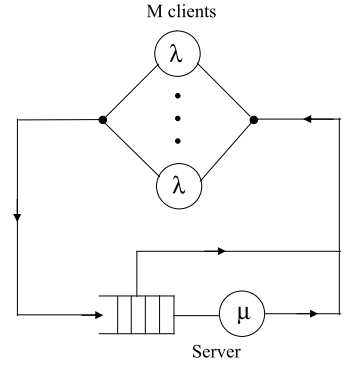
\includegraphics[scale=1]{figures/ex/cssystem.png}
\caption{Client-Server System}
\end{figure}

Client/Server con $M$ utenti. $\forall$ utente, in media dopo $\frac{1}{\lambda} s$ (EXP NEG) invia una richiesta al server. Il server esegue le richieste con FCFS. $\frac{1}{\mu} s$ è il tempo di servizio. Un utente genera una richiesta dopo che la precedente è stata servita. Ogni utente, indipendentemenete dagli altri, dopo un periodo di riflessione $(\frac{1}{\lambda})$, può quindi inviare le richieste al server. Gli utenti sono tuttavia impazienti e possono cancellare le richieste: a partire dall'invio delle richieste, dopo un tempo di durata media $\frac{1}{\gamma} s$, cancella la richiesta. Può cancellare solo se la richiesta NON sta venendo eseguita. Tempi di servizio, cancellazione e di riflessione sono rispettivamente i.i.d. e statisticamente indipendenti tra di loro; Quindi DTT, utilizzazione CPU, \dots

Modellazione di un sistema Web. Non è contemplata la possibilità che un utente si scocci e vada via. Condizioni di saturazione: Studio del sistema sotto-stress. $\max\{M\}$ per avere determinate prestazioni. Numero di utenti massimo che il server può sopportare, tollerare affinché si abbiano delle predeterminate prestazioni. $t\rightarrow \frac{1}{\lambda}$ per cliccare su un certo Hyperlink. 

Sistema reale Questo sistema reale descritto può essere modellato come una RETE DI CODE CHIUSA. Sistema a coda. Modello stocastico che rappresenta questo sistema reale descritto. Varie entità in gioco: \{\{utenti\}, server\}. Si parla di: \{tempi di riflessione, tempi di servizio, tempi di cancellazione\}. Server Web. Processo applicativo. Clienti + servitore + fila di attesa. Una rete di code è un insieme di code interconnesse tra di loro secondo una certa topologia. APERTA quando i clienti possono arrivare dall'esterno e partire verso l'esterno di questo sistema. CHUSA quando NON c'è la possibilità che arrivino dall'esterno o partano verso l'esterno. In tal caso il numero dei clienti è costante (Non si arriva e non si parte). Situazioni intermedie rendono il sistema non stabile. I blocchi di ritardo sono modellabili con delle code [$\mathord{\cdot}$/M/$\infty$]. Questa è una RETE DI CODE CHIUSA. $M=\cardinality{clienti}$. $M$ utenti nel sistema reale. Clienti + servitore. Un cliente si può trovare o nei blocchi di ritardo oppure nel sistema a coda. La presenza di un cliente nel blocco di ritardo rappresenta il fatto che nel sistema reale gli utenti possono avere un tempo di riflessione. Abbiamo $M$ unità di ritardo. Se un cliente è in un blocco di ritardo, il corrispondente utente nel sistema reale si trova in un periodo di riflessione. Il passaggio di un cliente dal blocco di ritardo verso il sistema a coda rappresenta il fatto che l'utente ha cliccato su un hyperlink: ha inviato una richiesta al server. Fila di attesa. Il passaggio di un cliente dalla fila di attesa verso il centro di servizio corrisponde al fatto che il server ha preso in considerazione la richiesta Web. Quando nel modello il cliente parte, andrà nuovamente nel blocco di ritardo. Il corrispondente utente nel sistema reale, avendo usufruito dell'erogazione del servizio, starà di nuovo pensando, scegliendo il successivo hyperlink da cliccare. C'è anche la possibilità che un cliente vada via dalla fila di attesa PRIMA ancora che venga servito. Ciò corrisponde alla situazione reale al fatto in cui un utente cancelli la propria richiesta in attesa, in coda. Possibilità che i clienti vadano via dalla fila di attesa. Anche quando un cliente va via dalla fila di attesa, giungerà nuovamente nei blocchi di ritardo. Modello stocastico che rappresenta bene il sistema reale.

Rete di code. Potrei risolverla con le tecniche adibite alla risoluzione di queste reti di code. Ma procederemo con i processi stocastici. Consideriamo il processo stocastico: $N(t)=\cardinality{clienti\ del\ sistema\ a\ tempo\ t}$ (Nel sistema a coda). Dinamica determinata dalle v.a.: \{tempi di riflessione, tempi di servizio, tempi di annullamento\}. Sono tutte v.a. exp-neg i.i.d. e statisticamente indipendenti tra di loro $\implies $ CMTC. DTT:

\begin{center}
\begin{tikzpicture}[->, >=stealth', auto, semithick, node distance=2.8cm]
\tikzstyle{every state}=[fill=white,draw=black,thick,text=black,scale=1]
\node[state]    (0)                     {$0$};
\node[state]    (1)[right of=0]   {$1$};
\node[state]    (2)[right of=1]   {$2$};
\node[state] (d) [right of=2] {\ldots};
\node[state]    (MM1)[right of=d]  {$M-1$};
\node[state]    (M)[right of=MM1]   {$M$};
\path
(0) edge[bend left]     node{$M\lambda$}         (1)
(1) edge[bend left]     node{$(M-1)\lambda$}         (2)
    edge[bend left,below]    node{$\mu$}            (0)
(2) edge[bend left]     node{$(M-2)\lambda$}           (d)
    edge[bend left,below]    node{$\mu+\gamma$}             (1)
(d) edge[bend left]         node{$(M-3)\lambda$}   (MM1)
	edge[bend left,below]   node{$\mu+2\gamma$}          (2)
(MM1)edge[bend left]    node{$(M-1)\lambda$}     (M)
     edge[bend left,below] node{$\mu+(M-2)\gamma$} (d)
(M) edge[bend left,below] node{$\mu+(M-1)\gamma$} (MM1);
\end{tikzpicture}
\end{center}

I clienti che NON si trovano nel sistema a coda saranno in una condizione di \underline{ARRIVO} nel sistema a coda. Il tempo che ci mette per uscire dal blocco di ritardo e giungere nel sistema a coda è $(\dots)\sim EXP-NEG(\lambda)$ i.i.d. indipendente dalle altre. Consideriamo uno stato non estremo. $0<i<M$. Supponiamo che al tempo $t$, $\underline{N(t)=i}=\cardinality{clienti\ in\ fila\ di\ attesa}+\cardinality{clienti\ nel\ centro\ di\ servizio}$. Avremo rispettivamente $i-1$ clienti in coda ed 1 nel centro di servizio. Se lo stato a tempo $t$ è i, avremo un certo numero $(M-i)$ in condizioni di arrivo. Se lo stato è i, la successiva transizione di stato potrà essere determinata da: un arrivo nel sistema a coda, quando finisce un servizio in corso, oppure a causa di un annullamento di una delle $(i-1)$ richieste pendenti. In questo caso, si avrà una transizione di stato (variazione di stato). $t \rightarrow$ successivo arrivo. Indichiamo al solito con $\xi_{R(t)}|_i\sim EXP ((M-i)\lambda) = \min\{(\dots)\}$, ovvero pari al minimo delle v.a. che rappresentano il tempo di arrivo residuo del k-esimo cliente nel blocco di ritardo (NO TEMPO DI INTERARRIVO!). Tempo che passa invece dall'istante $t$ al successivo completamento dell'erogazione del servizio è $\eta_{R(t)}|_i\sim EXP(\mu)$. Il tempo che passa dall'istante presente $t$ ed il successivo annullamento della richiesta è una v.a. definita in tal modo: $\theta_{R(t)}|_i\sim EXP[(i-1)\gamma]=\min\{(\dots)\}$, ovvero pari al minimo delle v.a. che rappresentano il tempo di annullamento residuo al tempo $t$. Ricordiamo: $\phi_i(t)\sim EXP(-q_{ii})$, ovvero il tempo di soggiorno nello stato $i$. Inoltre, $\Pr\{\phi_i(t)>\tau\}$, la sua CDF complementare, è pari alla probabilità che in $\tau$ NON ci sia nessun arrivo, NON ci sia la fine del servizio in corso e NON vi sia annullamento di una richiesta; il tutto condizionato con il fatto di trovarci nello stato $i$. Per indipendenza, essa è pari al prodotto delle rispettive probabilità, ovvero:

\[
	\Pr\{\phi_i(t)>\tau\} = [\Pr\{\xi_{R(t)} > \tau\ |\ i\}\Pr\{\eta_{R(t)} > \tau\ |\ i\}\Pr\{\theta_{R(t)} > \tau\ |\ i\}] =
\]
\[	
	= \e^{-(M-i)\lambda\tau}\e^{-\mu\tau}\e^{-(i-1)\gamma\tau} = e^{[\underline{-[(M-i)\lambda+\mu+(i-1)\gamma] = x]\tau}}
\]

Cosicché $(-q_{ii}=[x]) > 0$, ovvero abbiamo trovato la VELOCIT\`A TOTALE DI USCITA. Procediamo al solito modo:

\[
	\underline{\tau_{i,i+1}} = \frac{q_{i,i+1}}{-q_{ii}} = (\dots)
\]

dove $[-q_{ii}=[(M-i)\lambda+\mu+(i-1)\gamma]]$; il termine sottolineato è invece la probabilità che, lasciando lo stato $i$, migriamo verso lo stato $i+1$.

\[
	(\dots) = \Pr\{\xi_{R(t)} < \underline{\min\{\eta_{R(t)},\ \theta_{R(t)}\}}\} = (\dots)
\]

ove tale quantità rappresenta la probabilità che il successivo arrivo preceda il verificarsi dei due altri eventi. Tramite il teorema delle probabilità totali, otterremo alla fine:

\[
	(\dots) = \frac{(M-i)\lambda}{(M-i)\lambda+\mu+(i-1)\gamma} \implies
\]
\[
	\left\{
	\begin{aligned}
	&[q_{i,i+1} = (M-i)\lambda]\\
	&[q_{i,i-1} = \mu+(i-1)\gamma]
	\end{aligned}
	\right.
\]

Abbiamo quindi capito perché i tassi di transizione sono proprio questi. 

\[
	N(t)=0 \implies \underline{\phi_0(t)}\sim EXP(-q_{00}) =\underline{\xi_{R(t)}|_0} \sim EXP(M\lambda)
\]

$\implies \underline{-q_{00} = M\lambda}$. Se invece consideriamo lo stato $N(t)=M$ (tutti i clienti nel sistema a coda), avremo 0 clienti invece nel blocco di ritardo. La successiva transizione di stato sarà determinata o dall'annullamento di una richiesta o dalla fine dell'erogazione del servizio in corso:

\[
	\phi_M(t) = \min\{\eta_{R(t)}, \theta_{R(t)}\} \sim EXP((M-1)\gamma+\mu)
\]

$\implies -q_{MM} = (M-1)\gamma+\mu$. Quindi in realtà possiamo considerare valida la definizione di $-q_{ii}$ per $1<i\leq M$, in realtà.

CATENA \underline{\underline{ERGODICA}} $\iff$ OMOGENEA, IRRIDUCIBILE e $\cardinality{stati}<+\infty\iff$ numero di stati finito. Nel sistema a coda più di $M$ clienti NON ci possono essere $(\iff \cardinality{stati}<+\infty)$. 

CMTC tempo continuo, nascita e morte $\implies$

\[
	\left\{
	\begin{aligned}
	&[\pi_i=\pi_0 \lambda^i \frac{M!}{(M-i)!} \frac{1}{\prod_{k=0}^{i-1}{(\mu+k\gamma)}}]\\
	&\pi_0 = \frac{1}{1+\sum_{i=1}^M{\lambda^i \frac{M!}{(M-i)!} \frac{1}{\prod_{k=0}^{i-1}{(\mu+k\gamma)}}}}
	\end{aligned}
	\right.
\]

ove $\pi_0$ lo otteniamo con la condizione di NORMALIZZAZIONE. $i-1$ richieste pendenti ed un'altra in esecuzione nella CPU (del Server). $\rho$ è l'UTILIZZAZIONE, ovvero la frazione di tempo in media nella quale il servitore è impegnato a servire i clienti: $[\rho=1-\pi_0]$. Adesso dobbiamo valutare il throughput medio (throughput della CPU). Numero medio di richieste servite dalla CPU $\forall$ unità di tempo. Quando la CPU termina il servizio della richiesta, il cliente partirà dal centro di servizio. Applichiamo \underline{Little} ed otteniamo:

\[
	[\rho=\frac{\lambda_S}{\mu} \implies \lambda_S = \mu\rho = \mu(1-\pi_0)]
\]

Se consideriamo il prodotto $\pi_i[\mu+(i-1)\gamma]$, otteniamo la frequenza delle transizioni di questo tipo. Numero medio di volte che accade questa transizione $\forall$ unità di tempo. Consideriamo allora: $\underline{\pi_i\mu} + \underline{\pi_i(i-1)\gamma}$. Il primo termine sottolineato è la frequenza delle transizioni che portano da $i$ ad $i-1$ A CAUSA della fine di un servizio, mentre il secondo termine sottolineato rappresenta la frequenza delle transizioni $i\rightarrow i-1$ A CAUSA dell'annullamento di una richiesta. 

\[
	\left\{
	\begin{aligned}
	&[\lambda_S = \mu\pi_1 + \mu\pi_2 + \mu\pi_3 + \dots + \mu\pi_M = \mu(1-\pi_0) = \mu\rho]\\
	&[\lambda_R = \gamma\pi_2 + 2\gamma\pi_3 + 3\gamma\pi_4 + \dots + (M-1)\gamma\pi_M]
	\end{aligned}
	\right.
\]

Ove la seconda equazione rappresenta la velocità di partenza dei clienti dalla fila di attesa. Per trovare il numero medio di clienti in stato di riflessione, quindi, applichiamo nuovamente Little:

\[
	\bar{N}_R = \underline{(\lambda_S+\lambda_R)} \frac{1}{\lambda}
\]
\[
	\bar{N}_R = 0 \pi_M + 1\pi_{M-1} + 2\pi_{M-2} + \dots + M\pi_0
\]

Non è infatti difficile riconoscere ivi una media. Si può dimostrare che i due termini sono praticamente uguali e consistenti utilizzando le equazioni di BILANCIAMENTO LOCALE:

\[
	\pi_{i-1}(M-i+1)\lambda = \pi_i[(\mu+(i-1)\gamma)]
\]

Assumendo che le richieste NON possano essere cancellate, abbiamo che:

\[
	\underline{\E[R]} + \frac{1}{\lambda}
\]

Il primo termine sottolineato è il tempo medio di risposta, ove con $R$ intendiamo il tempo di risposta del sistema a coda, mentre il secondo addendo è al solito il tempo medio di riflessione. Un utente invierà una richiesta ogni $(\E[R]+\frac{1}{\lambda})$. Abbiamo $M$ richieste. $M$ utenti invieranno $M$ richieste alla seguente velocità:

\[
	(\frac{M}{\E[R]+\frac{1}{\lambda}}) = \underline{\lambda_S} = \mu\rho
\]

Dato che un utente NON può inviare una richiesta PRIMA che la precedente sia soddisfatta. Ove adesso il termine sottolineato rappresenta la velocità di arrivo delle richieste. Cosicché abbiamo:

\[
	\frac{M}{\mu\rho} = \E[R]+\frac{1}{\lambda} \implies \E[R] = \frac{M}{\mu\rho} -\frac{1}{\lambda} \implies \E[R]=\mathord{\cdot}{(M)}
\]

Se abbiamo 1 solo cliente $\iff M\rightarrow 1 \implies \E[R]=\frac{1}{\mu}$ NO fila di attesa. $M\uparrow (\mathord{\cdot}\to\infty) \implies \rho\to1 \implies \E[R]=(\frac{M}{\mu}-\frac{1}{\lambda})$, la quale quantità corrisponderebbe all'ASINTOTO OBLIQUO del grafico di $\E[R]$ in funzione di $M$.

L'asintoto viene in letteratura chiamato \textit{HEAVY LOAD asymptote}, mentre la retta ovviamente corrisponderebbe al \textit{LIGHT LOAD asymptote}. Il valore di $M$, $M^\star$ per il quale i due asintoti si incontrano, viene chiamato in letteratura \textit{SATURATION NUMBER}, ovvero il valore di $M=M^\star$ per il quale il sistema si considera in SATURAZIONE. Carico che può essere tollerato da un servizio, da un server:

\[
	\frac{1}{\mu} = \frac{M}{\mu} -\frac{1}{\lambda} \implies \frac{M}{\lambda} = \frac{1}{\mu}+\frac{1}{\lambda} \implies M^\star = (1+\frac{\mu}{\lambda})
\]

Tale valore rappresenta quindi il valore di $M$ per il quale il sistema è in saturazione. Se $\frac{1}{\lambda}=15 s$, e nel caso in cui $\frac{1}{\mu}=1 s$, abbiamo $\implies M^\star = 16 = 1+(15=\frac{\mu}{\lambda})$.

Ricordiamo che:

\[
	\underline{R(t) = \Pr\{X > t\}}
\]

è l'AFFIDABILIT\`A.

\subsection{RECAP}

M/M/1. Stato: $N(t) := \cardinality{clienti\ nel\ sistema\ a\ coda}$ (nell'intero sistema a coda). $N_q(t) := \cardinality{clienti\ in\ fila\ di\ attesa}$. CATENA DI MARKOV (OMOGENEA). Noto lo stato presente è possibile determinare l'evoluzione futura del processo in termini probabilistici, senza conoscere la storia passata (lo stato presente riassume tutta l'evoluzione passata). CATENE = stato discreto. Dell'evoluzione futura fa parte anche il tempo di soggiorno residuo $\phi_i(t) \sim EXP(-q_{ii})$. Se noto lo stato del processo nell'istante presente non riesco a determinare la distribuzione del tempo di soggiorno residuo, nel tempo in cui mi trovo, possiamo dire che NON riusciamo a determinare l'evoluzione futura. Evoluzione futura in termini probabilistici.

M/M/1. $\cardinality{clienti\ in\ fila\ di\ attesa}=\underline{N_q(t) = 0}$. Supponiamo vi siano 0 clienti (informazione che ho sullo stato presente del processo). Proviamo a determinare la distribuzione del tempo di soggiorno residuo in questo istante, MA non so se ci sono clienti nel centro di servizio. 

Supponiamo che vi sia un cliente nel centro di servizio (servitore occupato). Se termina quel servizio, si avrà una transizione di stato? NO. $\underline{\phi_0}(t)$ (0 clienti in fila di attesa). Se c'è 1 cliente, $\phi_0(t)\sim EXP(\lambda)$. Tempo di interarrivo residuo. Ma se non c'è nessuno, quella v.a. non sarà mica pari al tempo di interarrivo residuo. La transizione di stato si ha se arriva un cliente e ne arriva un altro. (Quindi se mettiamo insieme l'informazione invece riusciamo). Ma se includiamo quell'informazione torniamo alla precedente definizione di stato.

\section{RETI DI CODE}

Una rete dati di tipo switched può essere modellata mediante una rete di code. Queste code interagiscono tra di loro. Uno stream di pacchetti in partenza da una coda potrà andare a visitare un'altra coda dopo un merging con pacchetti provenienti da un'altra coda. [MERGING = POOLING]. Quindi una volta acceduti alla rete (superata la coda di accesso), si crea (si viene a creare) una correlazione tra i tempi di interarrivo dei pacchetti e quelli di trasmissione. Quindi viene meno l'ipotesi iniziale di indipendenza tra tempi di servizio e tempi di interarrivo. Adesso i tempi di servizio corrispondono ai tempi di trasmissione. Immaginiamo che i pacchetti arrivino alla rete con un processo di $\lambda$-POISSON. Nodo di accesso. Supponiamo che le lunghezze dei pacchetti siano v.a. equidistribuite statisticamente (i.d.), mutuamente indipendenti (con un certo valor medio), ed indipendenti dai tempi di interarrivo dei pacchetti al nodo di accesso. Tempi di trasmissione $\sim EXP(\mathord{\cdot})$. Data una certa capacità, le lunghezza dei pacchetti sono collegate ai tempi di trasmissione. Supponiamo che tempi di elaborazione e propagazione siano trascurabili. FCFS disciplina di coda. Serve però un'ipotesi aggiuntiva riguardo la dimensione dei buffer $(d=+\infty)$, ovvero illimitata.

Sistema reale: insieme dei due router con linee random (coda in serie). Il primo sistema è un M/M/1, per le ipotesi fatte. Si osservi il ramo che collega il primo centro di servizio con l'ingresso nel secondo buffer, e si effettuino delle analisi sulla eventuale dipendenza tra tempi di servizio e tempi di interarrivo. \`E evidente che le due grandezze sono in \textit{CORRELAZIONE}. Non posso quindi parlare di coda M/M/1 per il secondo sottosistema. A parte che non sappiamo che processo degli arrivi sia. Lo sapremo mediante teorema di \underline{BURKE}.

\begin{center}
\begin{figure}[H]
\centering
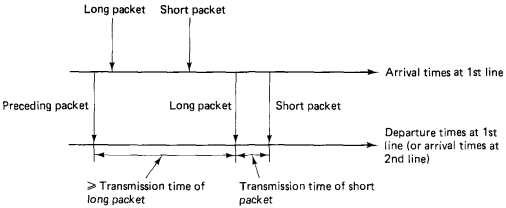
\includegraphics[scale=1]{figures/klnrk.png}
\caption{Timing Diagram of packet arrivals and departures completions in a system of two transmission lines in tandem} 
\end{figure}
\end{center}

Supponiamo che ad un certo istante termini la trasmissione di un pacchetto precedente. Poi, arrivi un pacchetto grande alla prima coda, il quale, trovandola vuota e notando disponibile il centro di servizio, ivi vi entra subito e viene iniziato il servizio (trasmissione). Finita la trasmissione di questo pacchetto, possiamo osservare che il tempo di interarrivo alla seconda coda (distanza temporale tra l'istante di arrivo del precedente pacchetto e l'istante di arrivo di questo), è risultato maggiore del tempo di trasmissione del pacchetto grande. Questo sarebbe già sufficiente per compromettere l'indipendenza. Si noti comunque che, se durante la trasmissione arriva un piccolo pacchetto alla prima coda, trovando il centro di servizio occupato, è costretto ad attendere in fila di attesa. Quando finirà la trasmissione del pacchetto grande, il piccolo potrà essere trasmesso. Ma a questo punto osserveremo un tempo di interarrivo (tra il grande ed il piccolo pacchetto) alla seconda coda praticamente uguale al tempo di trasmissione del piccolo pacchetto. Notiamo che vale: $\underline{t_{IA}\geq t_T}$, ovvero il tempo di interarrivo al secondo router è maggiore uguale del tempo di trasmissione nel primo router (in particolare sarà più grande se e solo se il secondo pacchetto trova la prima coda vuota (incluso il centro di servizio) al suo arrivo). Dal momento che nelle reti dati tipicamente avremo una lunghezza costante dei pacchetti, saranno quindi correlati anche i tempi di interarrivo al secondo sottosistema con i suoi tempi di servizio, dal momento che le lunghezze dei pacchetti influenzano i tempi di trasmissione, e quindi di servizio, anche se capacità dei link è differente tra i due. $\implies$ NO INDIPENDENZA. Leonard Kleinrock, il pioniere nella Ricerca delle Reti delle Code, ha risolto brillantemente questo problema. Andare a combinare (MERGING) su una certa coda flussi di pacchetti provenienti da altre code ha l'effetto di ripristinare l'indipendenza tra tempi di interarrivo a tempi di trasmissione. Se nel nostro esempio osserviamo al secondo router pacchetti di un altro router (nodo), non c'è più correlazione! Ripristino dell'ipotesi di INDIPENDENZA. La possibilità che accada questo evento dipende dal livello di comunicazione e di traffico! Più la rete è magliata (più merging di differenti flussi), e più è intenso il traffico, più è probabile che accadano eventi di questo tipo. La rete deve essere \textit{DENSAMENTE CONNESSA} ed il traffico deve essere intenso. Cosicché per una rete densamente connessa e per intensità di traffico medio-alta, possiamo ritenere valida la cosiddetta \textit{\textbf{APPROSSIMAZIONE DI INDIPENDENZA DI KLEINROCK}}. Intensità di traffico medio-alta inoltre! Possiamo mantenere sempre valida l'indipendenza tra tempi di interarrivo e tempi di trasmissione (servizio).

\subsection{RETE DI CODE APERTA}

Rete di code: insieme di code interconnesse tra di loro. Supponiamo di avere il seguente scenario:



Stiamo rappresentando con una rete di code un sistema di Elaborazione.

Clienti/Servitori/Fila di Attesa. Questa è la topologia della rete di code. Stiamo modellando un sistema di elaborazione. I clienti corrispondono alle richieste di esecuzione dei job (la presenza di un clientre in $\mu_1$ significa che si sta eseguendo quel job). I job stanno arrivando dall'esterno. Nodi alias stazioni di servizio. Il nodo 0 corrisponde al mondo esterno, dal quale possono arrivare i clienti. SINGLE CLASS \underline{OPEN}. Una rete si dice \underline{aperta} quando i clienti possono arrivare dall'esterno e fluire (partire) verso l'esterno. Per una CHIUSA (\underline{CLOSED}) è il contrario di quella aperta. Per una CHIUSA il numero di clienti è costantè (\textit{ISARITHMIC CONGESTION CONTROL}). $\exists M$ percorsi nella rete. Una rete di code, quando in essa i clienti arrivano esattamente se partono gli altri: 1 entra $\leftrightarrow$ 1 esce, può essere considerata chiusa. A volte possiamo volutamente limitare ad $M$ il numero di pacchetti che transitano. 

\underline{SINGLE CLASS OPEN}. Tornando al nostro caso, i clienti arrivando dall'esterno nel nostro sistema a coda, possono visitare solo il nodo 1 $\iff \underline{\underline{p_{01}=1}}$. Ma potrebbero $\exists(p_{0i}\neq 1)$. Leggi delle probabilità:

\[
	[p_{11}+p_{10}+p_{12}+p_{13}+p_{14} = 1]
\]

Similmente per gli altri nodi. Una volta visitato il nodo 2, il cliente potrà visitare soltanto il nodo 1. Questo vale anche per gli altri nodi 3-4! ($\iff [p_{21}=p_{31}=p_{41}=1]$. SINGLE CLASS = \{singola classe di clienti\}. Ma potrebbero esserci più classi di clienti. Per una rete di code con vari nodi definiamo:

\[
	[\underline{p_{ij} := ROUTING\ PROBABILITY}]
\]

o \underline{PROBABILIT\`A DI ROUTING}. (collegate ai protocolli di instradamento). Si potrebbero definire delle probabilità per differenti classi. Per altri stream potrei scegliere delle differenti destinazioni. Si modellino i vari stream nella rete ($\exists K$ classi ad esempio) come delle "classi di clienti". Sia: $N=\cardinality{nodi}$. Indichiamo con $K$ il vettore riga: $\underline{K} := (K_1,K_2,\ \dots,\ K_N)$, ove tale vettore rappresenta il numero di clienti NEI VARI NODI. Difatti, $K_i:=\cardinality{clienti\ al\ nodo\ "i"}$. E quindi: $K=\sum_{i=1}^N{K_i} := \cardinality{clienti\ nella\ rete}$. Definiamo: $[m_i\geq 1]:=\cardinality{servitori\ paralleli\ al\ nodo\ "i"}$. Indichiamo con $\mu_i$ la velocità del singolo servitore al nodo "i" (In generale possiamo avere velocità differenti per il nodo "i"). Noi considereremo servitori alla stessa velocità. Introduciamo il concetto di [Soluzione in forma PRODOTTO].

$p_{ij}$ = probabilità di routing $\implies p_{0,j}$ = probabilità che un cliente in arrivo dall'esterno vada a visitare il nodo $j$. Similmente, $p_{i,0}$ = probabilità che un cliente in partenza dal nodo $i$, lasci la rete. Cosicché: $pi_{i,0} = 1-\sum_{j=1}^N{p_{ij}}$. $\lambda_{0i}$ = velocità di arrivo dei clienti dall'esterno al nodo "i". Indichiamo con $\lambda$ la velocità totale di arrivo dei clienti dall'esterno $\iff \lambda=\sum_{i=1}^N{\lambda_{0i}}$. La velocità totale sarà tale che: $\lambda_{0i}=\lambda p_{0i}$. Indicando con $\lambda_i$ la velocità TOTALE di arrivo dei clienti al nodo $i$ e con $\lambda_j$ la velocità di partenza delle altre code, otteniamo:

\[
	[\lambda_i=\lambda_{0i}+\sum_{j=1}^N{\lambda_jp_{ji}}]
\]

con $i=1,2,\ \dots,\ N$. Dividendo membro a membro per $\lambda$ otteniamo:

\[	
	\frac{\lambda_i}{\lambda} = \frac{\lambda_{0i}}{\lambda} + \sum_{j=1}^N{\frac{\lambda_j}{\lambda}p_{ji}}
\]

con $i=1,2,\ \dots,\ N$. Queste sono le cosiddette \underline{EQUAZIONI DEL TRAFFICO}. Definiamo allora:

\begin{defn}{\textbf{Visit Ratio}}

Definiamo il VISIT Ratio come:

\[
	[e_i := \frac{\lambda_i}{\lambda}]
\]
\end{defn}

Esso rappresenta il numero medio di visite al nodo "i" $\forall$ arrivo dall'esterno. Quante volte un cliente IN ARRIVO DALL'ESTERNO visita il nodo "i" prima di lasciare la rete. Ad esempio:

\[	
	\lambda_i=20\ clienti/s,\ \lambda=2\ clienti/s,\ \frac{\lambda_i}{\lambda}=(10/2 = 5)\ clienti/s
\]

Diamo ora un'altra definizione:

\begin{defn}{\textbf{Service Demand}}

Definiamo $D_i$ service demand la quantità totale di servizio che in media un cliente richiede in un certo nodo:

\[
	\left\{
	\begin{aligned}
	&[e_i = p_{0i} + \sum_{j=1}^N{e_jp_{ji}}]\\
	&[D_i := e_i(\frac{1}{\mu_i})]
	\end{aligned}
	\right.
\]

\end{defn}

Si noti che $D_i$ è una quantità temporale!


Consideriamo la seguente rete di code: Due code a singolo router in serie e supponiamo che il processo degli arrivi al nodo "1" sia di $\lambda$-POISSON, che i tempi di servizio dei clienti alla prima ed alla seconda coda siano v.a. $(\dots)\sim EXP(\mu_1)$ per la prima e $(\dots)\sim EXP(\mu_2)$ per la seconda, mutuamente indipendenti ed \underline{indipendenti} dal processo degli arrivi alle code (tempi di interarrivo dei clienti alle code). QUESTE NON SONO RETI DATI! Ma generiche reti di code. Supponiamo $(d=+\infty)$ e disciplina di coda FCFS. Con le ipotesi viste la prima coda è M/M/1. Riguardo alla seconda coda, il processo degli arrivi dei clienti alla seconda coda corrisponde al tempo di partenza (al processo delle partenze dei clienti del nodo 1). Quindi è una $\mathord{\cdot}$/M/1 (Il processo degli arrivi NON può essere considerato, descritto indipendentemente dal resto della rete). Processo delle partenze. Questo fatto ci fa comprendere l'importanza di caratterizzare i processi delle partenze dei clienti delle code. Teorema di BURKE che fa la caso nostro:

\begin{thrm}{\textbf{Teorema di BURKE}}

Si consideri un sistema a coda M/M/1 $\lor$ M/M/m $\lor$ M/M/$(m=\infty)$. Sia $\lambda$ la velocità di arrivo dei clienti (processi degli arrivi dei clienti). Supponiamo di stare in condizioni di regime:

\begin{itemize}

\item{a)} Il processo delle partenze è \underline{di POISSON}, a velocità $\lambda$;
\item{b)} $\forall$ istante $t$, $\cardinality{clienti\ nel\ sistema}$ NON dipende dalla sequenza delle partenze fino a $t$. Esso dipende SICURAMENTE dagli arrivi che ci sono stati fino a $t$, SICURAMENTE dai tempi di servizio dei clienti che SONO stati effettivamente serviti;
\end{itemize}
\end{thrm}

Per dimostrarlo si dovrebbero utilizzare le CATENE DI MARKOV \textit{REVERSIBILI} (Ragionare andando nel verso opposto come tempo $\iff$ guardando l'evoluzione a ritroso).
Determinare la cosiddetta \textit{OCCUPANCY DISTRIBUTION}, ove intendiamo la probabilità che vi siano $K_1$ clienti nella "coda 1" e $K_2$ clienti nella "coda 2" a regime (probabilità congiunta):

\[
	\Pr\{K_1\ clienti\ nella\ "coda\ 1",\ K_2\ clienti\ nella\ "coda\ 2"\} =
\]
\[
	= \Pr\{K_1,K_2\} := \underline{\pi(K_1,K_2)}
\]

Notazione con pedici anche possibile. Distribuzione congiunta dei clienti nelle VARIE CODE. Una rete di code si dice STABILE se $\forall$ sistema a coda di cui si compone è STABILE. CONDIZIONE DI STABILIT\`A:

\[	
	[(\rho<1) \iff (\frac{\lambda}{\mu} < 1) \iff \lambda<\mu] \implies
\]
\[
	\implies
	\left\{
	\begin{aligned}
	&\rho_1=\frac{\lambda}{\mu_1} < 1 \iff \lambda<\mu_1\\
	&\rho_2=\frac{\lambda}{\mu_2} < 1 \iff \lambda<\mu_2
	\end{aligned}
	\right.
\]

Imposta la stabilità delle code e delle reti di code, utilizzo il teorema di BURKE. Sfruttiamo la parte a) del teorema. Processi degli arrivi in 2 di POISSON. Se guardiamo "2", isolatamente sarebbe un M/M/1 adesso (grazie a BURKE). Sfruttiamo adesso la parte b) di BURKE. Consideriamo le v.a. casuali che rappresentano il numero di clienti in "1" ed in "2":

\[
	\Pr\left\{
	\begin{aligned}
	&N_1(t) = K_1\\
	&N_2(t) = K_2
	\end{aligned}
	\right.
\]

Abbiamo $\{N_1(t),N_2(t)\},\ \forall t$. Risulta:

\[
	N_1(t) \neq \mathord{\cdot} N_2(t)
\]

grazie a Burke $\implies N_1(t),N_2(t)$ sono v.a. indipendenti $\implies$

\[
	\pi_{K_1,K_2} := \pi(K_1,K_2) = \pi(K_1)\pi(K_2)
\]

pari ovvero al prodotto delle due distribuzione marginali dei sistemi a coda visti in isolamento. Soluzione in FORMA PRODOTTO della OCCUPANCY DISTRIBUTION. In realtà i singoli sistema a coda NON stanno in isolamento! \`E una rete di code infatti. Riprendendo l'esempio delle M/M/1, abbiamo:

\[
	\{\lambda,\mu\} \implies \underline{\pi(K_1,K_2)} = [(1-\rho_1)\rho_1^{K_1}][(1-\rho_2)\rho_2^{K_2}]
\]

dove abbiamo: $\{(\rho_1=\frac{\lambda}{\mu_1}),\ (\rho_2=\frac{\lambda}{\mu_2})\}$. Ove abbiamo semplicemente utilizzato le espressioni trovate per la M/M/1. Allo stesso risultato si poteva arrivare senza sfruttare Burke ed analizzando con approccio Markoviano le seguenti reti di code, utilizzando una definizione di stato bidimensionale (multi-indice) (al tempo $t$). Sfruttiamo l'EQ. DI BILANCIAMENTO TOTALE dei flussi per una CATENA ERGODICA. Dovremo però aggiungere ovviamente la condizione di normalizzazione. Si arriva a scrivere:

\[
	\pi_{K_1,K_2} = (1-\frac{\lambda}{\mu_1})(1-\frac{\lambda}{\mu_2})(\frac{\lambda}{\mu_1})^{K_1}(\frac{\lambda}{\mu_2})^{K_2} =
\]
\[	
	= [\underline{((1-\frac{\lambda}{\mu_1})(\frac{\lambda}{\mu_1})^{K_1} = \pi_1(K_1))}][\underline{((1-\frac{\lambda}{\mu_2})(\frac{\lambda}{\mu_2})^{K_2} = \pi_2(K_2))}] = \underline{\pi(K_1)\pi(K_2)}
\]

Proviamo a sostituirle nelle equazioni di bilanciamento.

Giustificazione matematica. $\underline{(K_1,K_2)}$. Quindi ai fini della \underline{Occupancy Distribution}, la distribuzione congiunta è pari al prodotto delle distribuzioni marginali.

\subsection{Feed-Forward (Reti di code ACICLICHE)}

Tutte le reti di code che comprendono code del tipo: \{$\mathord{\cdot}$/M/1, $\mathord{\cdot}$/M/m, $\mathord{\cdot}$/M/$\infty$\} le quali ricevono arrivi sia da altre code della rete, sia dall'esterno, secondo processi di POISSON, e che non permettono a nessun cliente di ritornare ad una coda già visitata (SENZA CICLI), sono risolubili in forma prodotto. ACICLICHE $\iff \nexists$ CICLI. Per come sono fatte queste reti di code i processi degli arrivi sono di POISSON alle varie CODE.

\subsubsection{SEARCH ENGINE - MOTORI DI RICERCA}

Si consideri una porzione di rete in cui sono presenti tre motori di ricerca organizzati gerarchicamente in due livelli (vedi figura): a livello più alto e’ presente il motore MC, mentre a livello gerarchico più basso sono presenti i motori MA e MB. Gli utenti sono connessi al livello gerarchico più basso. Una richiesta di ricerca viene presentata da un generico utente al proprio motore. Questo, se dopo averla elaborata, non e’ in grado di soddisfarla, la reindirizza verso il motore MC che e’ sicuramente in grado di risolverla. Si assuma che:

\begin{itemize}

\item{i)} le richieste di ricerca da parte degli utenti del gruppo A siano presentate in accordo ad un processo di Poisson con parametro $\lambda_A\ req/min$;
\item{ii)} le richieste di ricerca da parte degli utenti del gruppo B siano presentate in accordo ad un processo di Poisson con parametro $\lambda_B\ req/min$;
\item{iii)} in ogni motore un unico processore elabori le richieste in modalità FCFS e con tempi che sono v.c. indipendenti distribuite secondo una ddp esponenziale negativa a valor medio pari, rispettivamente per i tre motori $M_A$, $M_B$, e $M_C$, a $T_A$ sec, $T_B$ sec e $T_C$ sec;
\item{iv)} una richiesta sia soddisfatta con probabilità $\alpha$ da un motore di livello basso;
\item{v)} sia trascurabile il tempo necessario ad inoltrare una richiesta al motore $M_C$.  

\end{itemize}

Calcolare:

\begin{itemize}

\item{a)} il fattore di utilizzazione del processore nel motore $M_C$;
\item{b)} il tempo medio di risoluzione di una richiesta;
\item{c)} il tempo medio di risoluzione di una richiesta da parte degli utenti del gruppo A. 
  
\end{itemize}

\begin{center}
\begin{figure}[H]
\centering
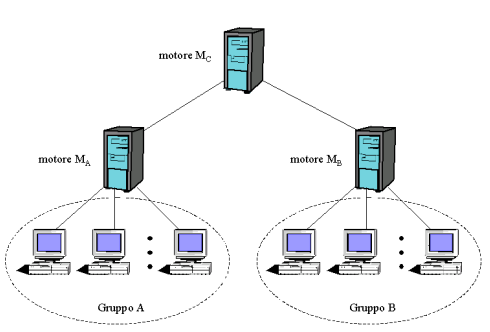
\includegraphics[scale=1]{figures/ex/se.png}
\caption{Hierarchical Search Engines}
\end{figure}
\end{center}

Risoluzione:

Tre motori di ricerca organizzati gerarchicamente in tre livelli. Gli utenti sono connessi al livello gerarchico più basso. $\{\lambda_A,\lambda_B\}\ req/min$, processi di POISSON. Richieste in modalità FCFS. Per quanto concerne i tempi di servizio, siamo dinanzi delle ddp esponenziali con i seguenti tempi di servizio medi, rispettivamente: $\{T_A, T_B, T_C\}s$. $M_C=?$ (fattore di utilizzazione). C'è da aggiungere un'ipotesi sulle dimensioni delle file di attesa: File di attesa illimitate $\iff (d=+\infty)$. Se qualcuna fosse un collo di bottiglia ci sarebbe scritta la dimensione $(\iff d<+\infty)$. Reti di code ACICLICHE. Processo degli arrivi dall'esterno di POISSON. Processo degli arrivi alle varie code di POISSON. Applicabile/applicato il teorema di BURKE. Abbiamo: $\{\mu_A=\frac{1}{T_A},\ \mu_B=\frac{1}{T_B},\ \mu_C=\frac{1}{T_C}\}$. Parametri della ddp esponenziale negativa. Popolazione illimitata $\iff (e=+\infty)$. Processo degli arrivi di POISSON. Rete ACICLICA $\iff$ feedforward network. Mi trovo dinanzi una rete di code. I processi degli arrivi sono di POISSON. Le reti A e B sono delle M/M/1. Viste in isolamento sono delle M/M/1. $\{K_A,\ K_B,\ K_C\}$ ci servono per definire la Occupancy Distribution (Burke + Splitting/Pooling). Code M/M/1 viste in isolamento $\iff$ grazie alla Soluzione in forma prodotto. Dobbiamo applicare le EQUAZIONI DEL TRAFFICO. La velocità di arrivo al sistema $M_C$ sarà:

\[
	\lambda_A(1-\alpha) + \lambda_B(1-\alpha) = (1-\alpha)(\lambda_A+\lambda_B) := \lambda_C
\]

I clienti NON si perdono! Se $\lambda_A$ arrivano nel primo sistema, $\lambda_A$ ne partiranno! Lo stesso dicasi per $M_C$. Per la STABILIT\`Adella rete di code dobbiamo imporre che $\forall$ sistema vi sia STABILIT\`A. Stabilità di ogni singolo sistema a coda:

\[
	\left\{
	\begin{aligned}
	&\rho_A = \frac{\lambda_A}{\mu_A}<1 \iff \lambda_A<\mu_A\\
	&\rho_B = \frac{\lambda_B}{\mu_B}<1 \iff \lambda_B<\mu_B\\
	&\rho_C = \frac{\lambda_C}{\mu_C}<1 \iff \lambda_C<\mu_C
	\end{aligned}
	\right.
\]

Analogamente... tre motodi di ricerca. Livello didattico. Nel calcolare $\lambda_C$ abbiamo anche risolto la prima domanda: $\rho_C=\frac{\lambda_C}{\mu_C}$, ovvero il FATTORE DI UTILIZZAZIONE del servitore nel nodo $M_C$. 

Tempo medio di risoluzione di una richiesta. L'arrivo nella rete di code di una richiesta corrisponde all'invio di una richiesta da parte di un utente. Tempo medio di risoluzione di una richiesta = tempo medio di permanenza nell'intero sistema. Clienti dall'esterno + Clienti in partenza $\leftarrow$ risoluzione di una richiesta. Si applichi Little:

\[
	[\bar{N}_{TOT} = \lambda_{TOT}\bar{R}] \implies \bar{R} = \frac{\bar{N}_{TOT}}{\lambda_{TOT}}
\]

$\bar{R}$ è quello che mi interessa. Sappiamo che: $\underline{\lambda_{TOT} = \lambda_A+\lambda_B}$, ovvero la velocità totale di arrivo dei clienti dall'esterno. Per un M/M/1 $\mathord{\cdot}(\lambda,\mu)$ il numero medio di clienti è: $(\bar{N}=\frac{\lambda}{\mu-\lambda})$. Lo dobbiamo però applicare ai vari sottosistemi. Somma dei numeri medi di clienti (a regime ovviamente):

\[
	[N_{TOT}=\bar{N}_A+\bar{N}_B+\bar{N}_C]\\
\]

sapendo che:

\[
	\left\{
	\begin{aligned}
	&\bar{N}_A = \frac{\lambda_A}{\mu_A-\lambda_A}\\
	&\bar{N}_B = \frac{\lambda_B}{\mu_B-\lambda_B}\\
	&\bar{N}_C = \frac{\lambda_C}{\mu_C-\lambda_C}
	\end{aligned}
	\right.
\]

Quindi abbiamo:

\[
	\bar{R} = \frac{N_{TOT}}{(\lambda_A+\lambda_B=\lambda_{TOT})}
\]

Per sapere invece il tempo medio di risoluzione di una richiesta da parte degli utenti del gruppo A $\iff R_A=?$, sapendo che per un M/M/1 vale:

\[
	\left\{
	\begin{aligned}
	&\bar{N}=\frac{\lambda}{\mu-\lambda}\\
	&\bar{T}=\frac{1}{\mu-\lambda}
	\end{aligned}
	\right.
\]

Allora si riconosce subito la media di una v.a.:

\[
	\bar{R}_A = \alpha[\frac{1}{\mu_A\lambda_A}] + (1-\alpha)[\frac{1}{\mu_A\lambda_A} + \frac{1}{\mu_C-\lambda_C}] =
\]
\[
	=  \frac{\alpha}{\mu_A-\lambda_A}+\frac{1}{\mu_A-\lambda_A}-\frac{\alpha}{\mu_A-\lambda_A}+\frac{1}{\mu_C-\lambda_C}-\frac{\alpha}{\mu_C-\lambda_C} =
\]
\[
	= [\frac{1}{\mu_A-\lambda_A}+\frac{(1-\alpha)}{\mu_C-\lambda_C}]
\]

Legittimo applicare Little al sottosistema $M_C$. Potremmo in realtà tentare un altro approccio. Potrei applicare Little a tutto il sistema ma considerando il numero di clienti del gruppo A. Sappiamo che:

\[
	\bar{N}_C = \frac{\lambda_C}{\mu_C-\lambda_C}
\]

Ma non stiamo diversificando i gruppi di clienti. La frazione di clienti A in $M_C$ è: $\frac{\lambda_A(1-\alpha)}{\lambda_C}$. Se facciamo questo rapporto, questa quantità corrisponderà proprio alla frazione dei clienti del gruppo A in $M_C$. Possiamo quindi scrivere la formula per sapere il numero medio di clienti del gruppo A in tutta la rete di code:

\[
	\bar{N}_{TOT,A} = ? = \frac{\lambda_A}{\mu_A-\lambda_A}+(\frac{\lambda_A(1-\alpha)}{\lambda_C})(\frac{\lambda_C}{\mu_C-\lambda_C}) = \frac{\lambda_A}{\mu_A-\lambda_A} + \frac{\lambda_A(1-\alpha)}{\mu_C-\lambda_C} =
\]
\[
	= \lambda_A[\frac{1}{\mu_A-\lambda_A}+\frac{(1-\alpha)}{\mu_C-\lambda_C}]
\]

Dobbiamo ora applicare Little:

\[
	\frac{\bar{N}_{TOT,A}}{\lambda_A} = \bar{R}_A = [\frac{1}{\mu_A-\lambda_A}+\frac{(1-\alpha)}{\mu_C-\lambda_C}]
\]

avendo considerato come velocità di arrivo solo $\lambda_A$, ovviamente.

\subsection{Reti di code CICLICHE}

Fino ad ora abbiamo visto le reti ACICLICHE $\iff$ Non permettiamo ad un cliente di visitare una coda già visitata. L'assenza di cicli è fondamentale per preservare la caratteristica di POISSON. Ciononostante esistono delle reti di code con CICLI per le quali continua comunque a valere la Soluzione in forma prodotto per la Occupancy Distribution. Reti di code con CICLO. Parliamo di rete aperta naturalmente. Due code $\mathord{\cdot}$/M/1 collegate in serie e con CICLO. Stiamo facendo l'ipotesi che i tempi di servizio siano v.a. distribuite esponenzialmente, mutuamente indipendenti e statisticamente indipendenti dai tempi di interarrivo dei clienti, distribuiti secondo $\lambda$-POISSON. 

\subsubsection{JACKSON NETWORK}

\underline{JACKSON NETWORK}. $\{p := p_1,\ p_2 := 1-p\}$. Ci favorisce la possibilità di calcolare la Occupancy Distribution sempre utilizzando la Soluzione in forma prodotto. Occupancy Distribution utilizzando una soluzione di stato bidimensionale $\{N_1(t),\ N_2(t)\}$. Processo stocastico. Due code $\mathord{\cdot}$/M/1. Fila di attesa illimitata $\iff (d=+\infty)$. Altrimenti non potrei parlare di M/M/1. Le ACICLICHE sono un sottoinsieme delle reti di JACKSON. Una rete di JACKSON senza cicli è una rete ACICLICA. Vale:

\[
	\lambda_1=\lambda+\lambda_2\alpha \stackrel{[\lambda_2=\lambda_1]}{=} \lambda+\lambda_1\alpha \implies
\]
\[
	\implies [\lambda_1 = \frac{\lambda}{1-\alpha} = \lambda_2]
\]

Dobbiamo imporre anche qui la STABILIT\`A dei singoli sottosistemi:

\[
	\left\{
	\begin{aligned}
	&\rho_1 := \frac{\lambda_1}{\mu_1} < 1 \iff \lambda_1<\mu_1\\
	&\rho_2 := \frac{\lambda_2}{\mu_2} < 1 \iff \lambda_2<\mu_2
	\end{aligned}
	\right.
\]

Adottiamo l'approccio precedente. Dobbiamo srivere le EQ. di bilanciamento totale dei flussi. Qui ovviamente NON possiamo applicare BURKE. I processi degli arrivi non sono di POISSON. Abbiamo scritto le equazioni di bilanciamento totale dei vari flussi. Dovrei risolvere il sistema aggiungendo la condizione di NORMALIZZAZIONE. Ricordiamo che: $\cardinality{stati}=+\infty$. Proviamo ad utilizzare questa distribuzione:

\[
	[\pi_{K_1,K_2} = \underline{(1-\frac{\lambda_1}{\mu_1})(\frac{\lambda_1}{\mu_1})^{K_1}} \underline{(1-\frac{\lambda_1}{\mu_2})(\frac{\lambda_2}{\mu_2})^{K_2}}]
\]

Ove i termini sottolineati sommano ad 1. Si può verificare che, dato che sostituite nella eq. di bilanciamento totale dei flussi essa è risolta $\iff$ è proprio quella la distribuzione. Prodotto delle distribuzioni marginali dei singoli sottosistemi, considerando che la loro distribuzione degli arrivi sia di POISSON, anche se in realtà non lo è! Sono sicuro che gli arrivi NON sono distribuiti secondo POISSON, ma i singoli sottosistemi, ai fini del calcolo della Occupancy Distribution, è proprio come se fossero degli M/M/1 in ISOLAMENTO! $\lambda$-POISSON autorizzati. Esempio di reti di code per le quali vale anche la Soluzione in forma prodotto $\rightarrow$ \underline{JACKSON NETWORK}

Dobbiamo formalizzare in generale queste particolari classi. Reti di Jackson, dal nome del ricercatore che ha studiato queste particolari reti di code. Ipotesi:

\begin{itemize}
\item{-)} Ci sono $N$ nodi: $\cardinality{nodi}=N$;
\item{-)} $\exists!$ classe di clienti. Non stiamo considerando più classi al momento;
\item{-)} RETE APERTA cosicché i clienti possono arrivare dall'esterno e partire verso l'esterno;
\item{-)} $\lambda_{0i}$-POISSON processi degli arrivi al nodo $i$ dall'esterno. $\lambda_{0i}$ può anche essere 0, ma affinché la rete sia aperte deve valere:

\[
	\exists i\ |\ (\lambda_{0i}>0) \neq 0
\]

Se $\lambda_{0i}=0$, la coda $i$ non prevede arrivi dall'esterno. Ricordiamo alcuni fatti:

\begin{itemize}

\item{$\lambda$}: velocità totale di arrivo dei clienti dall'esterno;
\item{$\lambda_{0i}=\lambda p_{0i}$}: velocità totale di arrivo dei clienti dall'esterno al nodo $i$;
\end{itemize}

Se $\forall i,\ \lambda_{0i}=0 \implies$ la rete è CHIUSA!
\item{-)}  Supponiamo che le file di attesa siano illimitate $\iff (d_i=+\infty\ \forall i)$. Al nodo $i$ ci sono $m_i$ servitori identici, dove $[m_i\geq 1]$. Velocità di servizio $\mu_i$. $\mu_i$ sia la velocità di servizio del generico servitore al nodo $i$. $(m_i=+\infty)$ è un caso contemplato. \{$\mathord{\cdot}$/M/1, $\mathord{\cdot}$/M/m, $\mathord{\cdot}$/M/$\infty$\};
\item{-)} i tempi di servizio sono distribuiti esponenzialmente, mutuamente indipendenti e statisticamente indipendenti dal processo degli arrivi dei clienti alla coda (considerando sempre una certa coda $i$);

\end{itemize}

Sostanzialmente, stiamo considerando $\mathord{\cdot}$/M/$m_i$, con $\{\frac{1}{\mu_i},\ \mu_i\ PAR\}$. Invece di considerare $m_i$ router identici nel sistema a coda $i$, possiamo ipotizzare la presenza di un unico servitore che operi con:

\[
	\mu_i(K_i) = \left\{
	\begin{aligned}
	&K_i\mu_i,\ K_i<m_i\\
	&\underline{m_i\mu_i},\ K_i\geq m_i
	\end{aligned}
	\right.
\]

\`E una velocità variabile governata da questa legge. $m_i$ servitori nel centro di servizio. La massima capacità di servizio possibile è per forza di cose il termine sottolineato. Possiamo considerare anche un servitore a velocità variabile, la cui velocità varia col numero di clienti presenti (nell'intero sistema a coda). Parliamo di \textit{LOAD DEPENDENT SERVICE-RATE} (LDSR). Discipline di coda per le varie code FCFS. \{$\mathord{\cdot}$/M/$m_i$), dove $(m_i\stackrel{CBE}{=}+\infty)$. Varie casistiche:

\[
	\left\{
	\begin{aligned}
	&m_i = 1\\
	&m_i > 1\\
	&m_i \leq +\infty
	\end{aligned}
	\right.
\]

Alla fine del servizio presso la coda $i$, un cliente va dalla coda "i" alla coda "j" con probabilità relativa di routing (un cliente, lasciando la coda "i", visita la coda "j" con probabilità $p_{ij}$), dove $i,j=1,2,\ \dots,\ (N=\cardinality{nodi})$, e potrà lasciare la rete con probabilità: $\underline{p_{i0}} = 1-\sum_{i=1}^N{p_{ij}},\ i=1,2,\ \dots,\ N$, ove il termine sottolineato rappresenta la probabilità di routing di un cliente da "i" verso l'esterno. PROBABILIT\`A DI ROUTING. Ricordiamo che il nodo 0 è l'esterno.

In una rete di Jackson le probabilità di routing sono uguali $\forall$ classe. Nelle BCMP generalmente sono differenziate in base alle varie classi. Ricordiamo le EQUAZIONI DEL TRAFFICO:

\[
	[\lambda_i = \lambda_{0i} + \sum_{j=1}^N{\lambda_j}{p_{ji}}]
\]

Adesso consideriamo il nodo $i$ per il quale $\exists i\ |\ m_i<+\infty$. $m$ servitori. Numero di router (servitori) finito. $m_i=\cardinality{servitori}$ (in parallelo). Possiamo calcolare il fattore di utilizzazione del generico servitore: $[\rho_i=\frac{\lambda_i}{m_i\mu_i}]$. "i" con $m_i$ servitori, tale per cui $(m_i>1)<+\infty$. $\rho_i<1$ per la stabilità della coda "i" (fattore di utilizzazione del generico servitore quando il carico è equamente distribuito). Dobbiamo imporre che:

\[
	\forall i\ | m_i<+\infty \implies \rho_i<1
\]

Notiamo infatti che se $m_i=+\infty$ allora la STABILIT\`A è sempre soddisfatta. \{$\mathord{\cdot}$/M/1, $\mathord{\cdot}$/M/m, $\mathord{\cdot}$/M/$\infty$\}. Tre tipologie di sistemi a coda per le JN. $\underline{K}=(K_1,K_2,\ \dots,\ K_N)\in\R^{N\times 1}$. Indichiamo con $K$ il vettore di stato, che considera il numero di clienti nelle varie code della JN. Mi interessa valutare la \underline{Occupancy Distribution}: $\pi(K_1,K_2,\ \dots,\ K_N)$ in condizioni di regime. Vi siano: \{$K_1$ clienti al nodo "1", $K_2$ clienti al nodo "2", \dots, $K_N$ clienti al nodo "N"\}. Per queste tipologie di reti di code la OD è esprimibile mediante Soluzione in forma prodotto $\implies$

\[
	\pi(K_1,K_2,\ \dots,\ K_N) = \pi(K_1)\pi(K_2)\ \dots\ \pi(K_N)
\]

Nelle JN i processi degli arrivi NON sono di POISSON. Possiamo però considerare i sistemi in isolamento.

\subsubsection{Exercise}

Un servizio di rete si basa su due server. Il processo stocastico secondo il 
quale si susseguono le richieste di esecuzione di un “job” da parte degli utenti 
può essere ben modellato da un processo di Poisson a velocità $\lambda$. In figura 1 è 
riportato lo schema che illustra la modalità di esecuzione dei job. Si noti 
come, dopo aver utilizzato il server \#1, con probabilità p1 un job lascia il 
sistema (job eseguito!), con probabilità $p2= 1-p1$, invece, un job utilizza il 
server\#2. Utilizzato il server\#2, un job viene nuovamente inserito nella coda 
del server\#1.

\begin{center}
\begin{figure}[H]
\centering
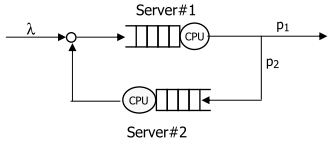
\includegraphics[scale=1]{figures/ex/jksnet.png}
\caption{Jackson Network}
\end{figure}
\end{center}

Si assuma che i singoli intervalli di tempo durante i quali viene utilizzato la 
CPU del server\#1 ed i singoli intervalli di tempo durante i quali viene 
utilizzata la CPU del server\#2 siano descritti da variabili casuali indipendenti 
e distribuite esponenzialmente a valor medio, rispettivamente, $\frac{1}{\mu_1}$ e $\frac{1}{\mu_2}$.  
Si assuma, inoltre, che i sistemi a coda in figura abbiano una capacità 
illimitata ed una disciplina di servizio di tipo FCFS.  
Si calcoli: 

\begin{itemize}
\item{a)} Il fattore di utilizzazione della CPU del server\#1; 
\item{b)} il valore medio del tempo di esecuzione di un job, a regime; 
\item{c)} il valore medio del tempo totale di CPU del server\#1 richiesto da un job, a 
regime; 
\item{d)} il valore medio del tempo totale di CPU del server\#2 richiesto da un job, a 
regime.

\end{itemize}

Risoluzione:

($\lambda$-POISSON) processi degli arrivi. $p_1$ che il job sia eseguito; $p_2=1-p_1$ che utilizzi il server 2. Se il job utilizza il server 2 ritorna in feedback all'ingresso di "1". $\{\{\lambda\},\{\mu_1,\mu_2\}\}$. $(d=+\infty)$, FCFS. Ci troviamo dinanzi una JN con code $\mathord{\cdot}$/M/1. Ma potrebbero anche essere \{$\mathord{\cdot}$/M/m, $\mathord{\cdot}$/M/$\infty$\}. M/M/1 in isolamento ai fini della OD. Definiamo con $\lambda_1$ velocità totale di arrivo dei clienti al nodo "1". Analogamente per "2", con $\lambda_2$. Applicando le equazioni del traffico troviamo:

\[
	\left\{
	\begin{aligned}
	&\lambda_1=\lambda+\lambda_2\\
	&\lambda_2=\lambda_1 p_2
	\end{aligned}
	\right. \implies \left\{
	\begin{aligned}
	&\lambda_1=\frac{\lambda}{1-p_2}\\
	&\lambda_2=\frac{\lambda}{(1-p_2=p_1)}p_2
	\end{aligned}
	\right.
\]

Dobbiamo imporre le Stabilità dei sottosistemi: $\implies$

\[
	\left\{
	\begin{aligned}
	&[\underline{\rho_1=\frac{\lambda_1}{\mu_1} = \frac{\lambda}{p_1\mu_1}}] < 1\\
	&[\underline{\rho_2=\frac{\lambda_2}{\mu_2} = \frac{\lambda p_2}{p_1\mu_2}}] < 1
	\end{aligned}
	\right.
\]

ove i termini sottolineati rappresentano il fattore di utilizzazione del server 1 e quello del server 2, rispettivamente. \underline{Little}. $\bar{N}=\bar{N}_1+\bar{N}_2$. Dove:

\[
	\left\{
	\begin{aligned}
	&\bar{N}_1 = \frac{\lambda_1}{\mu_1-\lambda_1} = \frac{\lambda}{p_1(\mu_1-\frac{\lambda}{p_1})} = \frac{\lambda}{p_1\mu_1-\lambda}\\
	&\bar{N}_2 = \frac{\lambda_2}{\mu_2-\lambda_2} = \frac{\lambda p_2}{p_1(\mu_2-\frac{\lambda p_2}{p_1})} = \frac{\lambda p_2}{p_1\mu_2-\lambda p_2} = \frac{\lambda}{\frac{p_1}{p_2}\mu_2-\lambda}
	\end{aligned}
	\right.
\]

Ricordiamo che $\lambda$ è la velocità totale di arrivo dei clienti dall'esterno. Dobbiamo quindi applicare Little: $\implies$ 

\[
	\bar{R} = \frac{\bar{N}_1+\bar{N}_2}{\lambda} = (\frac{1}{p_1\mu_1-\lambda} + \frac{1}{\frac{p_1}{p_2}\mu_2-\lambda})
\]

Quindi questo è il tempo medio di risposta. Dal punto di vista del tempo medio di risposta = tempo medio di permanenza, vi è un'equivalenza a due M/M/1 posti in serie, con velocità di servizio rispettivamente $\mu_1'=p_1\mu_1$ e $\mu_2'=\frac{p_1}{p_2}\mu_2$. RITARDO MEDIO il MEDESIMO, ma la distribuzione $\Pr\{R\leq t\}$ è DIFFERENTE!!

Calcoliamo le Service demand per i due nodi:

\[
	\left\{
	\begin{aligned}
	&D_1 = (\frac{1}{\mu_1}){(e_1=\frac{\lambda_1}{\lambda})} = \frac{1}{\mu_1} \frac{\lambda_1}{\lambda} = \frac{1}{\mu_1} \frac{\lambda}{p_1 \lambda} = \frac{1}{\mu_1 p_1}\\
	&D_2 = (\frac{1}{\mu_2})(e_2=\frac{\lambda_2}{\lambda}) = \frac{1}{\mu_2}\frac{\lambda p_2}{p_1}\frac{1}{\lambda} = \frac{1}{\mu_2}\underline{\frac{p_2}{p_1}}
	\end{aligned}
	\right.
\]

Dove $e_i$ rappresenta il numero medio di visite dall'esterno al nodo "i". Nel caso "2" ad esempio, il termine sottolineato indica $e_2 = \frac{p_2}{p_1}$. Notiamo che il nodo "1" verrà visitato sempre una volta in più prima di lasciare la rete: $+1 \implies \frac{p_2}{p_1}+1 = (\frac{1}{p_1})$. Potrei considerare: $\xi$ il numero totale di visite al server 1. $i-1$ volte visiti il nodo "2", e la volta successiva il cliente lascia la rete. Se $p_1=\Pr\{si\ lasci\ la\ rete\}$, allora vale:

\[
	\E[\xi] = \sum_{i=1}^{+\infty}{i\Pr\{\xi=i\}} = \sum_{i=1}^{+\infty}{ip_2^{i-1}p_1} =
\]
\[
	= p_1\sum_{i=1}^{+\infty}{ip_2^{i-1}} = p_1 \frac{1}{(1-p_2)^2} = p_1 \frac{1}{p_1^2} = \underline{\frac{1}{p_1}}
\]

(INDEPENDENT BERNOULLI TRIALS).


\subsection{Reti BCMP}

Reti di code \{CICLICHE, ACICLICHE, JACKSON\}. Per queste tipologie di code si ha una sola classe di clienti. Rete dati modellabile come rete di code, ma bisognerebbe differenziare le varie classi! $p_{ij} = \mathord{\cdot}(stream\ di\ pacchetti)$. Indici di prestazioni: \{ritardo medio\}. \underline{Reti di code BCMP} e teorema \underline{BCMP}. Va a definire una classe di reti di code per le quali vale ancora la Soluzione in forma prodotto per la Occupancy Distribution. Ma in questo caso i fattori del prodotto non corrispondono necessariamente alle distribuzioni marginali. Ma i fattori si ottengono a partire dall'analisi dei vari sistemi a coda visti in isolamento. Le BCMP comprendono le reti di JACKSON e quindi anche le ACICLICHE. C'è la possibilità di avere più classi di clienti $R$.

\begin{itemize}

\item{-)} $R=\cardinality{classi}$. Le classi possono essere APERTE o CHIUSE.

\begin{itemize}

\item{\textbf{APERTE}}: i clienti al loro interno possono partire dall'esterno ed arrivare dall'esterno;
\item{\textbf{CHIUSE}}: altrimenti
\end{itemize}

La BCMP è detta \textit{MIXED} se alcune classi sono aperte ed altre chiuse;

\item{-)} class switching possibile. Possibile che un cliente appartenente ad una certa classe, partendo da un nodo, visiti un certo nodo cambiando la sua classe;
\item{-)} $N=\cardinality{nodi}$. $p_{ir,js},\ r,s=1,2,\ \dots,\ (R=\cardinality{classi}),\ i,j=1,2,\ \dots,\ N=\cardinality{nodi}$ di reti di code. Si definirà quindi una \textit{matrice di routing}:

\begin{defn}{\textbf{Matrice di Routing}}

Per indicare le probabilità che un cliente appartenente ad una certa classe, partendo da un nodo, visiti un certo nodo cambiando la sua classe, si definisce:

\[
	\underline{\underline{P} := [p_{ir,js}]}
\]

\end{defn}

Tipicamente è una matrice SPARSA. A rigore sarebbe in realtà un tensore quadridimensionale. Se togliamo il class switching il tensore si ridurrebbe a 3 dimensioni.

\item{-)} Per quanto concerne la disciplina di coda, sino ad adesso abbiamo visto la FCFS, adesso ne sono consentite altre: \{\{PS, LCFS-PR, IS\}, FCFS\}. Ne spieghiamo qualcuna:

\begin{itemize}

\item{\textbf{PS} = \textit{processor sharing}}: \underline{tutti i clienti sono serviti contemporaneamente}, con time slicing;
\item{\textbf{LCFS-PR} = \textit{Last-Come-First-Served with Preemptive-Resume}}: Se un cliente viene servito ed arriva un altro cliente, vi è l'interruzione del servizio corrente ed il cliente corrente va in fila di attesa. Rientrerà nel servizio quando $\nexists$ clienti nel sistema a coda;
\item{\textbf{IS} = \textit{Infinite Server}}: Come suggerisce lo stesso nome, prevede INFINITI $(\infty)$ servitori! $\iff (m=+\infty)$ Come nell'M/M/$\infty$.

\end{itemize}

\end{itemize}

Vi è un'altra differenza (caratteristica aggiuntiva) riguardo la distribuzione dei tempi di servizio. Fino ad adesso abbiamo visto la distribuzione esponenziale. Adesso è permessa qualsiasi distribuzione purché la trasformata di Laplace della PDF sia razionale. COX ha dimostrato che qualunque distribuzione di v.a. si può approssimare sufficientemente bene mediante le seguenti reti di stadi: abbiamo una Rete di Stadi esponenziali. Il tempo di permanenza di un cliente in $\mu_i$ è distribuito esponenzialmente. Possiamo associare delle variabili casuali $\{\eta_1,\eta_2,\ \dots,\ \eta_n\}$ che sono tutte distribuite esponenzialmente $\iff \eta_i \sim EXP(\mu_i)\ \forall i=1,\ \dots,\ n$, ed indicano il tempo di permanenza in ciascuno stadio $i$-esimo. $\{a_i,b_i\}$ sono delle probabilità. La distribuzione associata all'attraversamento (al tempo di attraversamento) dell'intero sistema si chiama \textit{distribuzione di COX} e mediante essa possiamo approssimare (giocando opportunamente con il numero di stadi) sufficientemente bene una qualsiasi distribuzione. A questo punto il vincolo della trasformata di Laplace razionale della PDF non è più limitativo dal momento che la distribuzione di COX ha una TL della PDF razionale (PDF associata alla v.a. tempo di attraversamento).

Quindi possiamo pensare ad un unico servitore che rappresenti tutto il sistema. Il servitore è unico! Il servizio parte quando entra nel sistema e finisce quando il cliente esce dall'ultimo stadio. Solo alla fine un altro cliente va al servizio. In alcuni casi è ammessa una velocità del servizio che dipenda dal numero di clienti nella coda (M/M/m), o dal numero di clienti di una CERTA CLASSE nella coda.

(Probabilità di routing). La disciplina NON è a priorità! Ancora non la stiamo esaminando (interruzioni e senza interruzioni). Per queste reti che prevedono le forme prodotto NON è possibile.
Consideriamo il caso di rete BCMP aperta (\textit{OPEN-BCMP}). Vediamo che i processi degli ARRIVI sono ammesssi in questa rete. Consideriamo due casi, due possibilità:

\begin{itemize}

\item{\textit{\underline{CASO 1}}}: i clienti arrivano alla rete da un'unica sorgente, con tempi di interarrivo indipendenti e distribuiti esponenzialmente. Il Rate di arrivi $(\lambda)$ può dipendere dal numero di clienti $K$ nella rete $\iff \lambda=\lambda(K)$. \underline{Se $[\lambda\neq\lambda(K)]$} (si riferisce al rate di arrivo), \newline
\underline{avremo un processo di POISSON omogeneo}. Un cliente in arrivo visiterà il nodo $i$ in classe $r$ con probabilità $p_{0,ir}$ (giungendo dall'esterno). Ovviamente dovrà valere il seguente vincolo:

\[
	[\sum_{i=1}^N{\sum_{r=1}^R{p_{0,ir}=1}}]
\]

\item{\textit{\underline{CASO 2}}}: Se non facessi delle semplificazioni dovrei trattare delle sottocatene di Markov ergodiche. Eviteremo quindi il class switching. Supponiamo che non vi sia CS quindi. In tal caso si ha un processo degli arrivi $\forall$ classe di clienti. La velocità di arrivo $\lambda_r$ (indicizzata su $r$) potrà dipendere da $K_r \implies \lambda_r=\lambda_r(K_r),\ r=1,2,\ \dots,\ R$. Se $\lambda_r\neq\lambda_r(K_r)$ avremo un processo di POISSON omogeneo per la classe $r$.
\end{itemize}

Con le BCMP si può benissimo modellare un \textit{J2EE}, con Studio di Affidabilità e Disponibilità annesso. Quindi nel \underline{primo} caso abbiamo un unico processo degli arrivi, mentre nel \underline{secondo caso} non abbiamo class switching ed abbiamo un processo degli arrivi differente $\forall$ classe della rete. $K_r=\cardinality{clienti\ della\ classe\ r}$. Tipi di nodi ammessi nella BCMP: Nodi: \{\underline{type 1}, \underline{type 2}, \underline{type 3}, \underline{type 4}\}.

\begin{itemize}

\item{\underline{type 1}}: FCFS node. Coda con tempi di servizio distribuiti esponenzialmente con lo stesso valor medio (SAME $\frac{1}{\mu_i}$) per tutte le classi. La velocità di servizio $(\mu_i)$ può dipendere dal numero di clienti totali nella coda (nel sistema a coda). LOAD DEPENDENT SERVICE-RATE (LDSR) possibile. Può servire per modellare dispositivi I/O, HDD. Lo utilizzeremo per modellare tempi di accodamento e trasmissione dei router. Considereremo quindi: \{$\mathord{\cdot}$/M/$m_i$, \underline{FCFS}\};

\item{\underline{type 2}}: PS node (processor sharing). Utilizzato per modellare le CPU. Code con servitore unico e disciplina PS. Tutti i clienti sono serviti contemporaneamente. Sono possibili distribuzioni dei tempi di servizio diverse per classi diverse. Differenza rispetto al type 1. E qui non ci deve essere per forza l'esponenziale \{\underline{DSD} for \underline{DSC}\}. Vale sempre il vincolo sulle TL della PDF dei tempi di servizio. La velocità di servizio per una classe può dipendere dal numero di clienti nel nodo od anche dal numero di clienti di quella classe nel nodo. (Anche qui LDSR possibile);

\item{\underline{type 3}}: Detto IS (\textit{Infinite Server}) node oppure \textit{Delay Node}, perché solitamente utilizzato per modellare il ritardo (ritardo di elaborazione). Tutto quello scritto per il \underline{type 2} vale anche per il \underline{type 3}. Code del tipo: $\mathord{\cdot}$/G/$\infty$. Sempre un servitore a disposizione. In fila di attesa NON c'è mai nessuno. (Infiniti servitori $\implies \nexists$ fila di attesa). \`E come se non ci fosse alcuna disciplina;

\item{\underline{type 4}}: LCFS-PR (LCFS with Preemptive Resume). Coda con un unico servitore con quella disciplina di servizio. Contempliamo quindi le \{$\mathord{\cdot}$/G/1 - LCFS-PR\}. Unico servitore con quella disciplina di coda.

\end{itemize}

\subsubsection{Teorema BCMP}

Andiamo direttamente ad una versione semplificata del teorema BCMP (\textit{Baskett, Chandy, Muntz and Palacios}). Versione semplificata. Serve per modellare le reti di dati. Consideriamo BCMP (reti di code) aperte con load independent arrival rate. Quindi sostanzialmente processi di arrivo omogenei. Reti BCMP aperte con $[\lambda\neq\lambda(K)] \implies$ processi degli arrivi omogenei sostanzialmente.

Consideriamo che le velocità di servizio siano tali che $[\mu_i\neq\mu_i(K)]$. Casi ovviamente estendibili. Consideriamo:

\[
	\left\{
	\begin{aligned}
	&N=\cardinality{nodi}\\
	&R=\cardinality{classi}\\
	&K_i=\cardinality{clienti\ totali\ nel\ nodo\ i}\\
	&K_{ir}=\cardinality{clienti\ di\ classe\ r\ nel\ nodo\ i}\\
	&\underline{K}=(K_1,K_2,\ \dots,\ K_N)\\
	&\left\{
	\begin{aligned}
	&K_i=\sum_{r=1}^R{K_{ir}}\\
	&K=\sum_{i=1}^N{K_i} = \sum_{i=1}^N{\sum_{r=1}^R{K_{ir}}}
	\end{aligned}
	\right.
	\end{aligned}
	\right.
\]

Con queste quantità, la Occupancy Distribution è uguale a:

\[
	\Pr\{\underline{K}\} = \pi(K_1,K_2,\ \dots,\ K_N) = \prod_{i=1}^N{\pi_i(K_i)}
\]

questa è la OD per questa OPEN-BCMP. $\pi_i(K_i)$ è caratterizzato in questo modo:

\[
	\pi_i(K_i) = \left\{
	\begin{aligned}
	&\underline{(1-\rho_i)\rho_i^{K_i}},\ type\ 1,\ type\ 2,\ type\ 4\\
	&\e^{-\rho_i}\frac{\rho_i^{K_i}}{K_i!},\ type\ 3
	\end{aligned}
	\right.
\]

Per quanto concerne l'equazione che presenta il termine sottolineato, è bene specificare che abbiamo una restrizione sul type 1: è necessario avere esclusivamente un unico servitore ($\underline{m_i=1\ \forall i}$). La formula ricorda tanto la M/M/1. Ma vale anche per type (1,2,4). Reti: $\mathord{\cdot}$/M/$(1=m_i)$. Per la terza invece abbiamo reti $\mathord{\cdot}$/G/$\infty$. $\rho_i$ è il fattore di utilizzazione del nodo $i$. Vale: $\rho_i := \sum_{r=1}^R{\rho_{ir}}$. ($\forall$ classe di servizio), Se ho $m_i$ servitori nel type 1, $\pi_i(K_i)$ avrà la stessa espressione trovata per la M/M/$m_i$ $(\lambda_i,\mu_i)$. Le velocità di arrivo le calcoliamo con le \underline{EQUAZIONI DEL TRAFFICO}. Considerando $(m_i=1)$, dobbiamo imporre che $(\rho_i<1)$ per la STABILIT\`A della CODA. Anche per il type 1 con più servitori $(m_i\geq 1)$, avremo: $\rho_i=\frac{\lambda_i}{m_i\mu_i}$ nel caso $m_i\geq 1$. Quindi:

\[
	\rho_{ir} = \left\{
	\begin{aligned}
	&\frac{\lambda_{ir}}{\mu_i},\ type\ 1,\ \mu_i\neq\mu_{ir}\\
	&\frac{\lambda_{ir}}{\mu_{ir}},\ type\ \{2,3,4\},\ (\mu_i=\mu_{ir}) = \mathord{\cdot}(IDX\ r)
	\end{aligned}
	\right.
\]

Nel secondo caso infatti (seconda equazione), le distribuzioni dei tempi di servizio possono essere differenti per le varie classi. Ricordiamo che vale: $[\underline{\lambda_i}=\sum_{r=1}^R{\lambda_{ir}}]$, differenziando ed includendo rispetto alle varie classi.  Il termine sottolineato rappresenta la velocità \underline{totale} di arrivo al nodo $i$.

\subsection{RECAP}

[BCMP $\supset$ JACKSON $\supset$ ACICLICHE]. $\pi_i(K_i)$, reti \{$\mathord{\cdot}$/M/1, $\mathord{\cdot}$/G/1-PS, $\mathord{\cdot}$/G/1-LCFS-PR\}. Per queste code, ai fini dell'Occupancy Distribution, si comportano come se fossero delle M/M/1 in isolamento ($1=m_i$ servitori $\forall i$). Nel type 1 abbiamo la FCFS, mentre nel type 2, type 4 non abbiamo quella disciplina di coda! \`E come se ai fini del calcolo della OD, avessimo invece proprio la disciplina FCFS. Si comportano proprio come se fossero M/M/1 in isolamento.

Per quanto riguarda il secondo caso, per un M/M/$\infty$ abbiamo $[\e^{-\rho_i}\frac{\rho_i^{K_i}}{K_i!}]$. Ma vale sostanzialmente per tempi di servizio non distribuiti esponenzialmente (per le $\mathord{\cdot}$/G/$\infty$). La motivazione è collegata proprio al teorema BCMP. Tornando al primo caso, ipotizziamo una rete di code BCMP con un processo degli arrivi dall'esterno che NON dipenda dal carico (Stiamo considerando un processo degli arrivi di POISSON omogeneo). Il BCMP vale anche se c'è un solo sistema a coda! Consideriamo $\mathord{\cdot}$/M/1. Adesso sono sicuro che mi trovo dinanzi una M/M/1. Adesso i processi degli arrivi sono di POISSON. Per il \underline{type 2}, M/G/1-PS. Stesso discorso per il \underline{type 4}. Le formule trovata per un M/M/1, sono valide anche per un \{\underline{M/G/1-PS}, {M/G/1-LCFS-PR}\}, ove i termini sottolineati si riferiscono rispettivamente a code del tipo \underline{type 2} e \underline{type 4}.


\section{Reti di dati}

Ulteriore passaggio verso la modellazione. Obiettivo: modellare una rete di dati switched. Consideriamo $(i\rightarrow j)$. Ci saranno 4 componenti di ritardo su questo link. Dobbiamo considerare:

\begin{itemize}

\item{-)} tempi di accodamento in $i$;
\item{-)} tempi di trasmissione su questo link;
\item{-)} tempi di propagazione;
\item{-)} tempi di elaborazione

\end{itemize}

Modellando queste componenti di ritardo per il link $(i\rightarrow j)$, consideriamo nel primo blocco sicuramente $\mathord{\cdot}$/M/1 e agli ultimi due blocchi utilizzeremo rispettivamente: \{$\mathord{\cdot}$/G/$\infty$ e $\mathord{\cdot}$/G/$\infty$\}.
I sistemi a coda sono dei modelli per modellare il ritardo.

Virtual Circuit (a commutazione di pacchetto). Per un certo flusso la ROTTA sarà sempre la stessa. Stiamo immaginando qui di avere 3 flussi: $\{X_{s1}, X_{s2}, X_{s3}\} \leftarrow$ velocità di arrivo. Per il link $(i\rightarrow j)$ abbiamo il flusso di pacchetti $s_1-s_2 \implies X_{s_{i-j}} = X_{s1}+X_{s2}$. A questo punto, per valutare $\lambda_{ij}$, dobbiamo trovare la somma delle $X_s$ estesa a tutti gli stream $S$ che attraversano il link $(i\rightarrow j)$:

\[
	[\underline{\lambda_{ij}} = \sum_{stream\ s\ in\ (i,j)}{X_s}]
\]

$X_{si}$ è il rate (velocità) del flusso $i$-esimo. La rete Internet è a commutazione di pacchetto ma di tipo Datagram (Rotte non sempre le stesse). Per le DATAGRAM: $f_{ij}(s_1)X_{s,1}$ rappresenta la Velocità di arrivo, considerando le opportune frazioni dei pacchetti. Qui per calcolare le velocità di arrivo totale dobbiamo considerare le seguenti formule:

\[	
	\underline{\lambda_{ij}} = \sum_{stream\ s\ in\ (i,j)}{f_{ij}(s)X_s}
\]

ove la somma è estesa al solito a tutti gli stream che attraversano il link $(i\rightarrow j)$. Biforcazione o fork possibile.

Velocità di arrivo totale dei vari link sia su una VC che su una DATAGRAM. Entrambe a commutazione di pacchetto. Rete di code BCMP. Versione semplificata del teorema per modellare una rete di dati come una rete di code. Modellare ogni link della rete con il seguente schema:




Ipotesi sul sistema reale. Rete BCMP (più flussi) $\implies$ ($\forall$ flusso $\exists$ classe associata ad esso $\iff (s\rightarrow r)$). Sia $R=\cardinality{flussi\ di\ pacchetti}$. Rete BCMP con $R$ classi di clienti. Consideriamo il generico flusso $s$, al quale corrisponde una certa velocità $X_s \impliedby (s\rightarrow X_s)$. Per quanto concerne le velocità totali abbiamo: $\underline{\lambda_{0,r}}$ è la velocità di arrivo dall'esterno dei clienti di classe $r$; $\lambda_{0,hr}$ è la velocità di arrivo dall'esterno dei clienti di classe $r$ alla coda di ingresso $h$ della rete; $p_{0,hr}$ è la probabilità che un cliente dall'esterno di classe $r$ vada verso la coda $h$. Immaginiamo che $h$ sia il nodo di ingresso $\implies p_{0,hr}=1$:

\[
	X_s=\lambda_{0,r} \impliedby [\lambda_{0,r}p_{0,hr} = \underline{\lambda_{0,hr}}]
\]

Difatti quella probabilità è 1 per quella coda che rappresenta il nodo di ingresso. $\nexists$ biforcazioni all'ingresso della rete. Per applicare il teorema BCMP dovremo imporre che questi pacchetti arrivino secondo un processo di POISSON. Un'altra ipotesi riguarda i tempi di trasmissione. Nel primo blocco modelliamo il ritardo di accodamento e quello di trasmissione. Dobbiamo ipotizzare che i tempi di trasmissione siano distribuiti esponenzialmente (Con la stessa distribuzione per tutte le classi). Parametro $(\frac{1}{\mu_{ij}})$ come valor medio. Supponiamo che i buffer del router siano molto grandi $(d=+\infty)$ da poter ritenersi illimitati. Valga l'approssimazione di Kleinrock. Indipendenza tra i tempi di interarrivo e tempi di servizio. (Reti magliate ed intensità di traffico medio-alta). Vale quando la rete è abbastanza magliata e intensità di traffico medio-alta. Con queste ipotesi possiamo applicare il teorema BCMP. I due successivi blocchi di ritardo modellano il tempo di propagazione e di elaborazione (quest'ultimo è il router $j$) (ADN). Per elaborazione si intende il ritardo per decidere il routing. Il router analizzerà i vari link e si occuperà di decidere consultando le tabelle di forwarding. Il tempo di propagazione si trascura solitamente. Al posto dell'$\mathord{\cdot}$/M/1 andrebbe bene un $\mathord{\cdot}$/M/$\infty$. Anche se non siamo vicini alla distribuzione esponenziale per le lunghezze dei pacchetti, tutto alla fine va ancora bene. Applichiamo quindi le formule BCMP. Sia: $\bar{R}$ il tempo medio di attraversamento della rete da parte di un pacchetto. \underline{POOLING} di tutti i flussi che attraversano lo stesso link. Abbiamo: $\bar{R}=\frac{N}{\gamma}$, ove abbiamo posto $\gamma:=\sum_{tutti\ gli\ stream\ s}{X_s}$ ovvero la velocità totale di arrivo dei pacchetti. Dato che abbiamo a che fare con valor medi... indichiamo inoltre con \{$\E[T_{ij}^p],\ \E[T_{ij}^e]\}$ rispettivamente il valor medio del tempo di propagazione ed il valor medio del tempo di elaborazione, entrambi sul link $(i\rightarrow j)$. Sfruttando le formule dell'M/M/1 e di Little otteniamo:

\[
	\bar{N}_{ij} = \frac{\lambda_{ij}}{\mu_{ij}-\lambda_{ij}} + \lambda_{ij}\E[T_{ij}^p] + \lambda_{ij}\E[T_{ij}^e]
\]

Abbiamo trovato il numero medio di pacchetti sul link $(i,j) \implies \bar{N}=\sum_{(i,j)}{\bar{N}_{ij}}$. Dividiamo per la velocità totale di arrivo dei pacchetti $(\gamma)$ e troviamo $\bar{R}$. Sempre per il fatto della forma prodotto. (M/M/1) in isolamento (BCMP TH.). Se introduco un modello M/G/$\infty$, un po' di errore lo commetto. Le formule che ottengo per l'M/G/$\infty$ sono analoghe a quelle M/M/$\infty$.

\begin{thrm}{\textbf{$\bar{R}_{path}$}}

Per calcolare questa quantità, dovrei considerare tutti i link associati a questo percorso:

\[
	\bar{R}_{path} := [\sum_{link(i,j)\ lungo\ path}{\frac{1}{\mu_{ij}-\lambda_{ij}}}] + \E[T_{ij}^p + \E[T_{ij}^e]]
\]

\end{thrm}

Vale per tutte le classi! $(\forall r=s)$. Qualunque sia la sua classe. Tanto è inglobata nelle varie quantità $(\mu_{ij},\ \lambda_{ij})$. 


\subsection{Exercise}

Consider the network in the figure below. There are four sessions: ACE, ADE, BCEF and BDEF 
sending Poisson traffic at rates $\{100,\ 200,\ 500,\ 600\}\ pkt/min$, respectively. Packets lengths are 
exponentially distributed with mean $1000\ bits$. All transmission lines have capacity $50\ kbits/s$, 
and there is a propagation delay of $2\ msec$ on each line. Using the Kleinrock independence 
approximation, 

\begin{itemize}

\item{a)} find the average number of packets in the system, the average delay per packet (regardless of 
session) and the average delay per packet of each session; 
\item{b)} derive the CTMC that can be used to find the approximate delay distribution related to the 
packets belonging to the ACE session

\end{itemize}

\begin{center}
\begin{figure}[H]
\centering
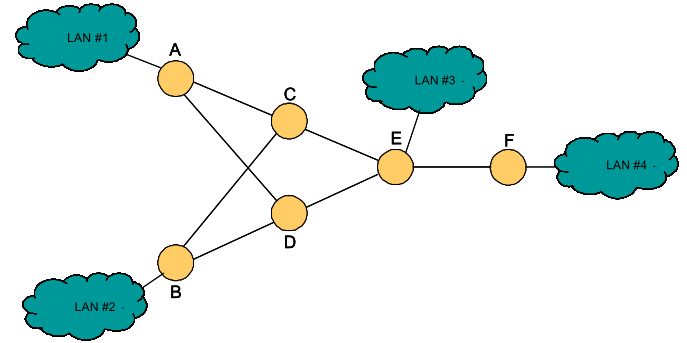
\includegraphics[scale=0.8]{figures/ex/mdn.png}
\caption{Data Network}
\end{figure}
\end{center}

Flussi in realtà bidirezionali. Ma a livello didattico concentriamoci nel caso NON DUPLEX ($\iff$ Flussi unidirezionali). Abbiamo varie sessioni:

\[
	\left\{
	\begin{aligned}
	&ACE, 1\\
	&ADE, 2\\
	&BCEF, 3\\
	&BDEF, 4
	\end{aligned}
	\right.
\]

Quattro servizi che generano pacchetti alle seguenti velocità. $\{100,200,500,600\}\  [pkt/min]$. $\mathit{L}=1000\ bit$ (lunghezza pacchetti), $C=50\ kbps$. $\E[T_{ij}^p]=dp=2ms$ (propagation delay, PD). ($\forall ij$. Qualunque sia il link $i,j$). Il PD è in realtà una costante, non un valor medio. Supponiamo quindi che tutti i link siano alla stessa velocità. Supponiamo valida l'approssimazione di Kleinrock. 4 flussi di pacchetti $\iff$ 4 sessioni di comunicazioni. Numeriamo le sessioni e calcoliamo:

\[
	\left\{
	\begin{aligned}
	&X_1 = (\frac{100}{60} = \frac{5}{3})\ pkt/s\\
	&X_2 = (\frac{200}{60} = \frac{10}{3})\ pkt/s\\
	&X_3 = (\frac{500}{60} = \frac{25}{3})\ pkt/s\\
	&X_4 = (\frac{600}{60} = 10)\ pkt/s
	\end{aligned}
	\right.
\]

Ci serve andare a calcolare le velocità totali di arrivo sui VARI link attraversati. 

\[
	\left\{
	\begin{aligned}
	&\lambda_{AC}=X_1\\
	&\lambda_{CE}=X_1+X_3=10\ pkt/s\\
	&\lambda_{AD}=X_2\\
	&\lambda_{BD}=X_4=10\ pkt/s\\
	&\lambda_{DE}=X_2+X_4=\frac{40}{3}\ pkt/s\\
	&\lambda_{BC}=X_3\\
	&\lambda_{EF}=X_3+X_4=\frac{55}{3}\ pkt/s
	\end{aligned}
	\right.
\]

Dobbiamo andare a considerare la velocità di servizio su ogni link. Ci troviamo dinanzi $\mathord{\cdot}$/M/1. Ma anche relativi ai router dei blocchi $\mathord{\cdot}$/G/$\infty$. Dividiamo $\frac{C}{\mathit{L}}=\mu_{ij}=(\frac{50000}{1000}=50)\ pkt/s$. Dobbiamo calcolare il $\gamma$ (velocità totale di arrivo dei clienti):

\[
	\gamma=\sum_{i=1}^4{X_i}=\frac{70}{3}\ pkt/s
\]

in quanto abbiamo 4 flussi diversi. Con $\bar{N} \simeq 1.84\ pkt$ pacchetti, abbiamo quindi:

\[
	\bar{R}=\frac{\bar{N}}{\gamma}=\frac{1.84}{70/3\ pkt/s} = \frac{3(1.84)}{70} msec\ (millisec)
\]

(poco credibile oggi). Dobbiamo ora calcolare il ritardo medio $\forall$ stream (per i vari stream). Per le varie sessioni ($\bar{R}_{path}$ formula), abbiamo:

\[
	\bar{R}_p=[50ms,\ 53ms,\ 87ms,\ 90ms]
\]

$\Pr\{R\leq t\}$, dove $R$ è il ritardo, tempo di attraversamento della rete.

Distribuzione del ritardo. Supponiamo di voler determinare la distribuzione del ritardo dei pacchetti associati alla sessione ACE. CMTC che con uno stato assorbente può essere utilizzata per modellare il ritardo $(ACE=AC+CE)$ (link attraversato):



Distribuzione di ritardo = tempo di permanenza di un pacchetto nella rete in questione. Abbiamo trascurato i ritardi di elaborazione. $\mathord{\cdot}$/M/1, che tiene conto dei ritardi di accodamento + il ritardo di trasmissione. Presso il nodo "C" arriveranno pacchetti anche dal nodo "B" (da un altro stream) (BCEF). Determinare la distribuzione del tempo di risposta in una rete di code aperta. C'è un metodo per approssimare questa distribuzione (del tempo di risposta), e si basa sulla conoscenza della distribuzione del tempo di risposta relativa ai vari sottosistemi di cui la rete si compone. Reti di code di JACKSON. Tempo di risposta = tempo di attraversamento. Vogliamo approssimare questa distribuzione (del tempo di risposta). \`E possibile andare a derivare da questa rete di JACKSON una CMTC con \underline{stato assorbente}. Il \underline{time-to-absorption} (la sua distribuzione), rappresenta un'approssimazione del tempo di risposta della rete. Se è ACICLICA (rete di JACKSON senza CICLI) si ha una coincidenza tra TTA e tempo di risposta della rete.
Consideriamo questa rete CICLICA:

\begin{center}
\begin{figure}[H]
\centering
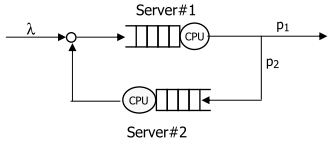
\includegraphics[scale=1]{figures/ex/jksnet.png}
\caption{Jackson Network}
\end{figure}
\end{center}

Due $\mathord{\cdot}$/M/1. Questo metodo si basa sulla conoscenza delle distribuzioni dei vari tempi di risposta dei singoli sottosistemi di cui si compone la rete. M/M/1. $R$ = tempo di permanenza. Sappiamo che: $R \sim EXP(\mu-\lambda)$. $F(t)\ CDF$, quindi la CDF del tempo di risposta in un M/M/1 è:

\[
	F(t)=\Pr\{R\leq t\} = 1-\e^{-(\mu-\lambda)t}
\]

Sulla base di queste conoscenze, possiamo dedurre, ricavare la seguente CMTC:

\begin{center}
\begin{tikzpicture}[->, >=stealth', auto, semithick, node distance=3cm]
\tikzstyle{every state}=[fill=white,draw=black,thick,text=black,scale=1]
\node[state]    (1)                     {$1$};
\node[state]    (2)[right of=1]   {$2$};
\node[state]    (C)[below of=1]   {$C$};
\path
(1) 
    edge[bend left]     node{$(\mu_1-\lambda_1)p_2$}     (2)
    edge[bend right,left]    node{$(\mu_1-\lambda_1)p_1$}      (C)
(2) edge[bend left]                node{$(\mu_2-\lambda_2)\underline{1}$} (1);
\end{tikzpicture}
\end{center} 

con: $\{\{C\},\{1,2\}\}$ rispettivamente come Stato assorbente e Stati transitori. Lo STARTING STATE è lo stato 1, ovvero lo stato dalla quale evolve la CMTC. $R\sim EXP(\mu-\lambda)$. Rappresenta la permanenza del cliente sul sistema. Tempo di permanenza di un determinato cliente. In particolare, il tempo di soggiorno della CMTC in questo stato corrisponde al tempo di permanenza nel primo M/M/1. ($R_1\sim EXP(\mu_1-\lambda_1)$). Il tempo di soggiorno della catena nello stato 2 rappresenta il tempo di permanenza del cliente nel sistema nel sistema a coda 2 ($R_2\sim EXP(\mu_2-\lambda_2)$). Se invece lasciasse la rete, si avrebbe una transizione verso lo stato assorbente \{C\}. Il TTA qui corrisponde al ritardo del cliente in questa rete (tempo di permanenza). Se riesco a determinare la distribuzione del TTA per questa catena riesco a determinare proprio il tempo di permanenza nella mia rete. Ma è un'approssimazione questa, in quanto abbiamo dei cicli! Quindi i processi degli arrivi NON sono di POISSON. 

\[
	\underline{\Pr\{T_a\leq t\}} \simeq \underline{\Pr\{R\leq t\}}
\]

ove il LHS sottolineato rappresenta $\pi_C(t)$ in TRANSITORIO, mentre il RHS sottolineato rappresenta la distribuzione del ritardo nella mia rete. A quanto pare vi è un'approssimazione possibile. Per trovare $\pi_C(t)$ si può procedere con il metodo della trasformata di Laplace, diversamente ci sono dei programmi di simulazione e non. Si richiami il concetto di affidabilità:

\[
	\Pr\{R>t\} = 1-\underline{\pi_0(t)} = 1-\Pr\{R\leq t\}
\]

\subsection{Response-Time Blocks (RTB)}

Li utilizziamo per trovare queste distribuzioni. Blocchi mediante i quali costruiamo le CMTC con stati assorbenti. Dobbiamo considerare tanti blocchi quante sono le componenti di ritardo.

\begin{itemize}

\item{\textbf{RTB \textit{M/M/1}}}: Ci sono quindi anzitutto quelle per la M/M/1 $(\lambda,\mu)$, ove per stabilità deve valere: $(\lambda<\mu)$. Il RTB per questo sistema è il seguente:

\begin{center}
\begin{tikzpicture}[->, >=stealth', auto, semithick, node distance=3cm]
\tikzstyle{every state}=[fill=white,draw=black,thick,text=black,scale=2]
\node[state]    (IN)                     {$IN$};
\node[state]    (OUT)[right of=IN]   {$OUT$};
\path
(IN) edge[bend left]     node{$(\mu-\lambda)$}     (OUT);
\end{tikzpicture}
\end{center}

Lo stato IN rappresenta il fatto che il cliente è entrato nella coda. Il tempo di soggiorno nello stato \{IN\} rappresenta il ritardo nella rete. \{OUT\} = \{partenza del cliente nella coda\}. (Tante serie di blocchi quanti sono i nodi in gioco):

\[
	\underline{F(t)} = 1-\e^{-(\mu-\lambda)t}
\]

Ove il termine sottolineato rappresenta la CDF del tempo di risposta. Lo stato \{OUT\} rappresenta la partenza del cliente. OUT nel precedente esercizio era \{2,C\}=OUT. In tali casi saranno da pesare le velocità di uscita complessive (con probabilità eventualmente, corrispondenti alle cosiddette probabilità di routing);

\item{\textbf{RTB \textit{M/M/$\infty$}}}: Il tempo di soggiorno nella mia catena corrisponde al tempo di servizio $\iff \nexists$ code nella M/M/$\infty$. (infiniti servitori, NO fila di attesa). 

\begin{center}
\begin{tikzpicture}[->, >=stealth', auto, semithick, node distance=3cm]
\tikzstyle{every state}=[fill=white,draw=black,thick,text=black,scale=2]
\node[state]    (IN)                     {$IN$};
\node[state]    (OUT)[right of=IN]   {$OUT$};
\path
(IN) edge[bend left]     node{$\mu$}     (OUT);
\end{tikzpicture}
\end{center}

Tempo di risposta corrisponde al tempo di servizio:

\[
	F(t) = \Pr\{R\leq t\}=1-\e^{-\mu t}
\]

\{IN\} rappresenta quindi lo stato di permanenza nel mio sistema;

\item{\textbf{RTB \textit{M/M/m}}}:

Per ultimo, ma non di importanza, abbiamo l'RTB di una M/M/m:

\begin{center}
\begin{tikzpicture}[->, >=stealth', auto, semithick, node distance=3cm]
\tikzstyle{every state}=[fill=white,draw=black,thick,text=black,scale=2]
\node[state]    (IN)                     {$IN$};
\node[state]    (OUT)[right of=IN]   {$OUT$};
\path
(IN) edge[bend left]     node{$\frac{\mu m (1-\rho)}{m(1-\rho)+C}$}     (OUT);
\end{tikzpicture}
\end{center}

ove $C$ è la C di ERLANG, ovvero la probabilità di accodamento;

\end{itemize}

Ma lo stato OUT può corrispondere allo stato IN di un altro blocco! Se effettivamente OUT è l'uscita della rete sarà assorbente, altrimenti NO.

Adesso consideriamo la rete precedente. Quella è la rete di code che modella la sessione ACE sostanzialmente:

\begin{center}
\begin{tikzpicture}[->, >=stealth', auto, semithick, node distance=3cm]
\tikzstyle{every state}=[fill=white,draw=black,thick,text=black,scale=1]
\node[state]    (A)                     {$A$};
\node[state]    (AC)[right of=A]   {$AC$};
\node[state]    (C) [right of=AC]                    {$C$};
\node[state]    (CE)[right of=C]   {$CE$};
\node[state]    (OUT)[right of=CE] {$OUT$};
\path
(A) edge[bend left]     node{$\mu-\lambda_AC$}     (AC)
(AC) edge[bend left]     node{$\frac{1}{d_AC}$}     (C)
(C) edge[bend left]     node{$\mu-\lambda_CE$}     (CE)
(CE) edge[bend left]     node{$\frac{1}{d_{CE}}$}     (OUT);
\node at ($(OUT)+(0,-0.8)$) {stato ASSORBENTE};
\end{tikzpicture}
\end{center}

Il nodo E interfaccia i pacchetti verso la LAN 3. (\underline{Rete ACICLICA}). Trascuriamo il ritardo di elaborazione, al solito. Velocità elevatissima! A volte si può ritenere legittimo trascurare il ritardo di accodamento e trasmissione della LAN di destinazione! Molto veloce! TTA in tal caso coincide esattamente con il ritardo di attraversamento (tempo di attraversamento) della rete, dal momento che la rete è ACICLICA.